\documentclass[xcolor={table}]{beamer}
\usepackage{fleqn}
\usepackage{graphicx}
\usepackage{coordsys} %for \numbline commander

%Setup appearance:
\usetheme{Darmstadt}
\usefonttheme[onlylarge]{structurebold}
\setbeamerfont*{frametitle}{size=\normalsize,series=\bfseries}
\setbeamertemplate{navigation symbols}{}
\setbeamertemplate{bibliography item}{[\theenumiv]}

% Standard packages
\usepackage[english]{babel}
\usepackage[latin1]{inputenc}
\usepackage{times}
\usepackage[T1]{fontenc}
\usepackage{multirow}
\usepackage{subfigure}
\usepackage{pbox}
\usepackage{arydshln}
\usepackage{pifont}
\usepackage{cancel}
\usepackage{rotating} % for sideways headings

% Source Code packages
\usepackage{algorithm2e}
\usepackage{algorithmic}

\DeclareSymbolFont{extraup}{U}{zavm}{m}{n}
\DeclareMathSymbol{\varclub}{\mathalpha}{extraup}{84}
\DeclareMathSymbol{\varspade}{\mathalpha}{extraup}{85}
\DeclareMathSymbol{\varheart}{\mathalpha}{extraup}{86}
\DeclareMathSymbol{\vardiamond}{\mathalpha}{extraup}{87}

\def\<{\langle}
\def\>{\rangle}

%%% This section command that adds a big page with section dividers
\usepackage{xifthen}% provides \isempty test
\newcommand{\SectionSlide}[2][]{
	\ifthenelse{\isempty{#1}}
		{\section{#2}\begin{frame} \begin{center}\begin{huge}#2\end{huge}\end{center}\end{frame}}
		{\section[#1]{#2}\begin{frame} \begin{center}\begin{huge}#2\end{huge}\end{center}\end{frame}}
}
%Extends the section slide to to include a shortened section title for the navigation bar as a second parameter
\newcommand{\SectionSlideShortHeader}[3][]{
	\ifthenelse{\isempty{#1}}
		{\section[#3]{#2}\begin{frame} \begin{center}\begin{huge}#2\end{huge}\end{center}\end{frame}}
		{\section[#1]{#2}\begin{frame} \begin{center}\begin{huge}#3\end{huge}\end{center}\end{frame}}
}

\newcommand{\refer}[1]{\footnote{#1}}
\newcommand{\GW}{\text{\textit{Guess-Who~}}}
\newcommand{\keyword}[1]{\alert{\textbf{#1}}\index{#1}}
\newcommand{\firstkeyword}[1]{\textbf{#1}\index{#1}}
\newcommand{\indexkeyword}[1]{\alert{\textbf{#1}\index{#1}}}
\newcommand{\featN}[1]{\textsc{#1}}
\newcommand{\featL}[1]{\textit{'#1'}}
 \newcommand{\ourRef}[1]{\ref{#1} $^{\text{\tiny[\pageref{#1}]}}$}
 \newcommand{\ourEqRef}[1]{\eqref{#1}$^{\text{\tiny[\pageref{#1}]}}$}
  
\DeclareMathOperator*{\argmax}{argmax}
\DeclareMathOperator*{\argmin}{argmin}


\title{Similarity-based Learning\\Sections $5.4, 5.5$}
	\author{John D. Kelleher and Brian Mac Namee and Aoife D'Arcy}
	\institute{}
	\date{}

\begin{document}
\begin{frame}
	\titlepage
\end{frame}
\begin{frame}
	 \tableofcontents
\end{frame}

\SectionSlideShortHeader{Handling Noisy Data}{Noisy Data}

 \begin{frame} 
\begin{figure}[htb]
       \begin{centering}
     		\includegraphics[width=0.7\textwidth]{./images/knn_fs_4_small.pdf}
     	  \caption{Is the instance at the top right of the diagram really \textit{noise}?}
	\label{fig:voronoidecboundB}
       \end{centering}
\end{figure}
\end{frame} 

\begin{frame} 
\begin{itemize}
\item The \alert{k nearest neighbors} model predicts the target level with the majority vote from the set of k nearest neightbors to the query $\mathbf{q}$:  
\end{itemize}

\begin{equation}
\centering
\mathbb{M}_{k}(\mathbf{q}) = \argmax_{l \in levels(t)} \sum_{i=1}^k \delta(t_i,l) 
\label{eq:knn}
\end{equation}
\end{frame} 


\begin{frame} 
\begin{figure}[htb]
	\begin{center}
	\includegraphics[width=0.7\textwidth]{./images/knn_fs_7_small.pdf}
	\end{center}
	\caption{The decision boundary using majority classification of the nearest 3 neighbors.}	
	\label{fig:knndecboundary3}
\end{figure}
\end{frame} 

\begin{frame} 
\begin{figure}[htb]
	\begin{center}
	\includegraphics[width=0.7\textwidth]{./images/knn_fs_8_small.pdf}
	\end{center}
	\caption{The decision boundary using majority classification of the nearest 5 neighbors.}	
	\label{fig:knndecboundary5}
\end{figure}
\end{frame} 


 \begin{frame} 
\begin{figure}[htb]
       \begin{centering}
       \includegraphics[width=0.7\textwidth]{images/knn_fs_9_small.pdf}
       \caption{The decision boundary when $k$ is set to 15.}
       \label{fig:bigk}
       \end{centering}
\end{figure}
\end{frame} 


\begin{frame} 
\begin{itemize}
\item In a distance \alert{weighted \textit{k} nearest neighbor} algorithm the contribution of each neighbor to the classification decision is weighted by the reciprocal of the squared distance between the neighbor $\textbf{d}$ and the query $\textbf{q}$:
\end{itemize}
\begin{center} 
\begin{equation}
 \frac{1}{dist(\mathbf{q}, \mathbf{d})^2}
\label{eq:reciprocalsquaredist}
\end{equation}
\end{center}
\begin{itemize}
\item The weighted \textit{k} nearest neighbor model is defined as: 
\end{itemize}
\begin{equation}
\mathbb{M}_{k}(\mathbf{q}) = \argmax_{l \in levels(t)} \sum_{i=1}^k \frac{1}{dist(\mathbf{q}, \mathbf{d_i})^2} \times \delta(t_i,l) 
\label{eq:weightedknn}
\end{equation}
\end{frame} 



 \begin{frame} 
\begin{figure}[htb]
       \begin{centering}
       \includegraphics[width=0.7\textwidth]{images/knn_fs_10_small.pdf}
       \caption{The weighted \textit{k} nearest neighbor model decision boundary.}
       \label{fig:weightedk}
       \end{centering}
\end{figure}
\end{frame} 

\SectionSlideShortHeader{Data Normalization}{Normalization}

 \begin{frame} 
\begin{table}[!tb]
\caption{A dataset listing the salary and age information for customers and whether or not the purchased a pension plan .}
\label{table:salaryAgeDataset}
\centering
\begin{footnotesize}
\begin{tabular}{ c  c  c  c }
\hline
\textbf{ID} & \textbf{Salary} & \textbf{Age} & \textbf{Purchased}\\
\hline
1 & 53700	& 41	& No \\
2 & 65300	& 37	& No \\
3 & 48900	& 45	& Yes \\
4 & 64800	& 49	& Yes \\
5 & 44200	& 30	& No \\
6 & 55900	& 57	& Yes \\
7 & 48600	& 26	& No \\
8 & 72800	& 60	& Yes \\
9 & 45300	& 34	& No \\
10 & 73200	& 52	& Yes \\
\hline
\end{tabular}
\end{footnotesize}
\end{table}
\end{frame} 


\begin{frame}
\begin{itemize}
	\item The marketing department wants to decide whether or not they should contact a customer with the following profile: \end{itemize}
\centerline{
$\left<\text{\featN{Salary}}=56,000,\text{\featN{Age}}=35\right>$
}
\end{frame}


 \begin{frame} [plain]
\begin{figure}[htb]
	\begin{center}
	\includegraphics[width=0.62\textwidth]{./images/knn_normalisation_1.pdf}
	\end{center}
	\caption{The salary and age feature space with the data in Table \ourRef{table:salaryAgeDataset} plotted. The instances are labelled their IDs, triangles represent the negative instances and crosses represent the positive instances. The location of the query $\left<\text{\featN{Salary}}=56,000,\text{\featN{Age}}=35\right>$ is indicated by the $?$.} 
	\label{fig:salaryAgePurchase}
\end{figure}
\end{frame} 

 \begin{frame} 
\begin{table}
\label{table:distancecomputationssalaryage}
\centering
\resizebox{\textwidth}{!}{\begin{tabular}{ c  c  c  c | r c | r c | r c}
\hline
\multicolumn{4}{c|}{~} & \multicolumn{2}{c|}{\textbf{Salary and Age}} & \multicolumn{2}{c|}{\textbf{Salary Only}} & \multicolumn{2}{c}{\textbf{Age Only}} \\
\textbf{ID} & \textbf{Salary} & \textbf{Age} & \textbf{Purch.} & \textbf{Dist.} &  \textbf{Neigh.}  & \textbf{Dist.} &  \textbf{Neigh.} & \textbf{Dist.} &  \textbf{Neigh.}\\
\hline
1 & 53700	& 41	& No  & 2300.0078 &	2 &	2300 & 2 & 6 & 4\\
2 & 65300	& 37	& No & 9300.0002 &	6	&9300	& 6& 	2&	2\\
3 & 48900	& 45	& Yes & 7100.0070 &	3	&7100	&3	&10	&6\\
4 & 64800	& 49	& Yes & 8800.0111 &	5	&8800	&5	&14&	7\\
5 & 44200	& 30	& No & 11800.0011 &	8	&11800	&8	&5	&5\\
\alert{6} & \alert{55900}	& \alert{57}	& \alert{Yes} & \alert{102.3914} &	\alert{1}	& \alert{100}	& \alert{1}	& \alert{22}	& \alert{9}\\
7 & 48600	& 26	& No & 7400.0055 &	4	& 7400	 &4 &	 9  & 	3\\
8 & 72800	& 60	& Yes & 16800.0186 &	9	& 16800 &	9	& 25 &	10\\
9 & 45300	& 34	& No & 10700.0000	&7	& 10700 &	7 &1	&1\\
10 & 73200	& 52	& Yes & 17200.0084 & 10 &	17200 &	10 & 17 &	8\\
\hline
\end{tabular}
}
\end{table}
\end{frame} 

\begin{frame}
\begin{itemize}
	 \item This odd prediction is caused by features taking different ranges of values, this is equivalent to features having different variances. 
	\item We can adjust for this using normalization; the equation for range normalization is:
\end{itemize}
\begin{equation}
a_i^{'} = \frac{a_i - min(a)}{max(a) - min(a)}\times \left(high-low \right) +low
\label{eq:rangenormalisationknn}
\end{equation}
\end{frame}

 \begin{frame} 
\begin{table}
\label{table:distancecomputationssalaryagenorm}
\centering
\resizebox{\textwidth}{!}{\begin{tabular}{ c  c  c  c | r c | r c | r c}
\hline
\multicolumn{4}{c|}{\textbf{Normalized Dataset}} & \multicolumn{2}{c|}{\textbf{Salary and Age}} & \multicolumn{2}{c|}{\textbf{Salary Only}} & \multicolumn{2}{c}{\textbf{Age Only}} \\
\textbf{ID} & \textbf{Salary} & \textbf{Age} & \textbf{Purch.} & \textbf{Dist.} &  \textbf{Neigh.}  & \textbf{Dist.} &  \textbf{Neigh.} & \textbf{Dist.} &  \textbf{Neigh.}\\
\hline
\alert{1}&	\alert{0.3276}	& \alert{0.4412}&\alert{	No} &\alert{0.1935}	&\alert{1}	&\alert{0.0793}	&\alert{2}	&\alert{0.17647}	&\alert{4}\\
2&	0.7276&	0.3235& No	&0.3260&	2&	0.3207	&6	&0.05882	&2\\
3&	0.1621	&0.5588&	Yes &0.3827&	5	&0.2448	&3	&0.29412	&6\\
4&	0.7103	&0.6765&	Yes &0.5115&	7	&0.3034	&5	&0.41176	&7\\
5&	0.0000	&0.1176&	No&0.4327&	6	&0.4069	&8	&0.14706	&3\\
6&	0.4034	&0.9118&	Yes&0.6471&	8	&0.0034	&1	&0.64706	&9\\
7&	0.1517	&0.0000&	No&0.3677&	3	&0.2552	&4	&0.26471	&5\\
8&	0.9862	&1.0000&	Yes&0.9361&	10	&0.5793	&9	&0.73529	&10\\
9&	0.0379	&0.2353&	No &0.3701&	4	&0.3690	&7	&0.02941	&1\\
10&	1.0000&	0.7647&	Yes &0.7757&	9	&0.5931	&10	&0.50000	&8\\
\hline
\end{tabular}
}
\end{table}
\end{frame} 


\begin{frame}
\begin{itemize}
	\item Normalizing the data is an important thing to do for almost all machine learning algorithms, not just nearest neighbor! 
\end{itemize}
\end{frame}


\SectionSlideShortHeader{Predicting Continuous Targets}{Cont. Targets}

 \begin{frame} 
	\begin{itemize}
		\item Return the average value in the neighborhood:
	\end{itemize}
\begin{equation}
\mathbb{M}_{k}(\mathbf{q}) =\frac{1}{k} \sum_{i=1}^k t_i
\label{eq:knncontpred}
\end{equation}
\end{frame} 


 \begin{frame} 
\begin{table}[htb]
\caption{A dataset of whiskeys listing the age (in years) and the rating (between 1 and 5, with 5 being the best) and the bottle price of each whiskey. }
\label{table:whiskeyPriceModel}
\begin{center}
\begin{footnotesize}
\begin{tabular}{cc}
		\hline
			\begin{minipage}{0.45\textwidth}
					\begin{tabular}[ht]{crrr} 
\textbf{ID}	 & \textbf{Age} & \textbf{Rating} & \textbf{Price}\\
\hline
1	&0	&2	&30.00\\
2	&12	&3.5	&40.00\\
3	&10	&4	&55.00\\
4	&21	&4.5	&550.00\\
5	&12	&3	&35.00\\
6	&15	&3.5	&45.00\\
7	&16	&4	&70.00\\
8	&18	&3	&85.00\\
9	&18	&3.5	&78.00\\
10	&16	&3	&75.00\\
\hline
					\end{tabular}
			\end{minipage}
			&
			\begin{minipage}{0.45\textwidth}
					\begin{tabular}[ht]{crrr} 
\textbf{ID}	 & \textbf{Age} & \textbf{Rating} & \textbf{Price}\\
\hline
11	&19	&5	&500.00\\
12	&6	&4.5	&200.00\\
13	&8	&3.5	&65.00\\
14	&22	&4	&120.00\\
15	&6	&2	&12.00\\
16	&8	&4.5	&250.00\\
17	&10	&2	&18.00\\
18	&30	&4.5	&450.00\\
19	&1	&1	&10.00\\
20	&4	&3	&30.00\\
\hline
				\end{tabular}
			\end{minipage}\\
\end{tabular}
\end{footnotesize}
\end{center}
\end{table}
\end{frame} 



 \begin{frame} 
\begin{table}[htb]
\caption{The whiskey dataset after the descriptive features have been normalized.}
\label{table:whiskeyPriceModelNorm}
\begin{center}
\begin{footnotesize}
\begin{tabular}{cc}
		\hline
			\begin{minipage}{0.45\textwidth}
					\begin{tabular}[ht]{crrr} 
\textbf{ID}	 & \textbf{Age} & \textbf{Rating} & \textbf{Price}\\
\hline
1	&0.0000	&0.25	&30.00\\
2	&0.4000	&0.63	&40.00\\
3	&0.3333	&0.75	&55.00\\
4	&0.7000	&0.88	&550.00\\
5	&0.4000	&0.50	&35.00\\
6	&0.5000	&0.63	&45.00\\
7	&0.5333	&0.75	&70.00\\
8	&0.6000	&0.50	&85.00\\
9	&0.6000	&0.63	&78.00\\
10	&0.5333	&0.50	&75.00\\
\hline
					\end{tabular}
			\end{minipage}
			&
			\begin{minipage}{0.45\textwidth}
					\begin{tabular}[ht]{crrr} 
\textbf{ID}	 & \textbf{Age} & \textbf{Rating} & \textbf{Price}\\
\hline
11	&0.6333	&1.00	&500.00\\
12	&0.2000	&0.88	&200.00\\
13	&0.2667	&0.63	&65.00\\
14	&0.7333	&0.75	&120.00\\
15	&0.2000	&0.25	&12.00\\
16	&0.2667	&0.88	&250.00\\
17	&0.3333	&0.25	&18.00\\
18	&1.0000	&0.88	&450.00\\
19	&0.0333	&0.00	&10.00\\
20	&0.1333	&0.50	&30.00\\
\hline
				\end{tabular}
			\end{minipage}\\
\end{tabular}
\end{footnotesize}
\end{center}
\end{table}
\end{frame} 


 \begin{frame} [plain]
\begin{figure}[htb]
	\begin{center}
	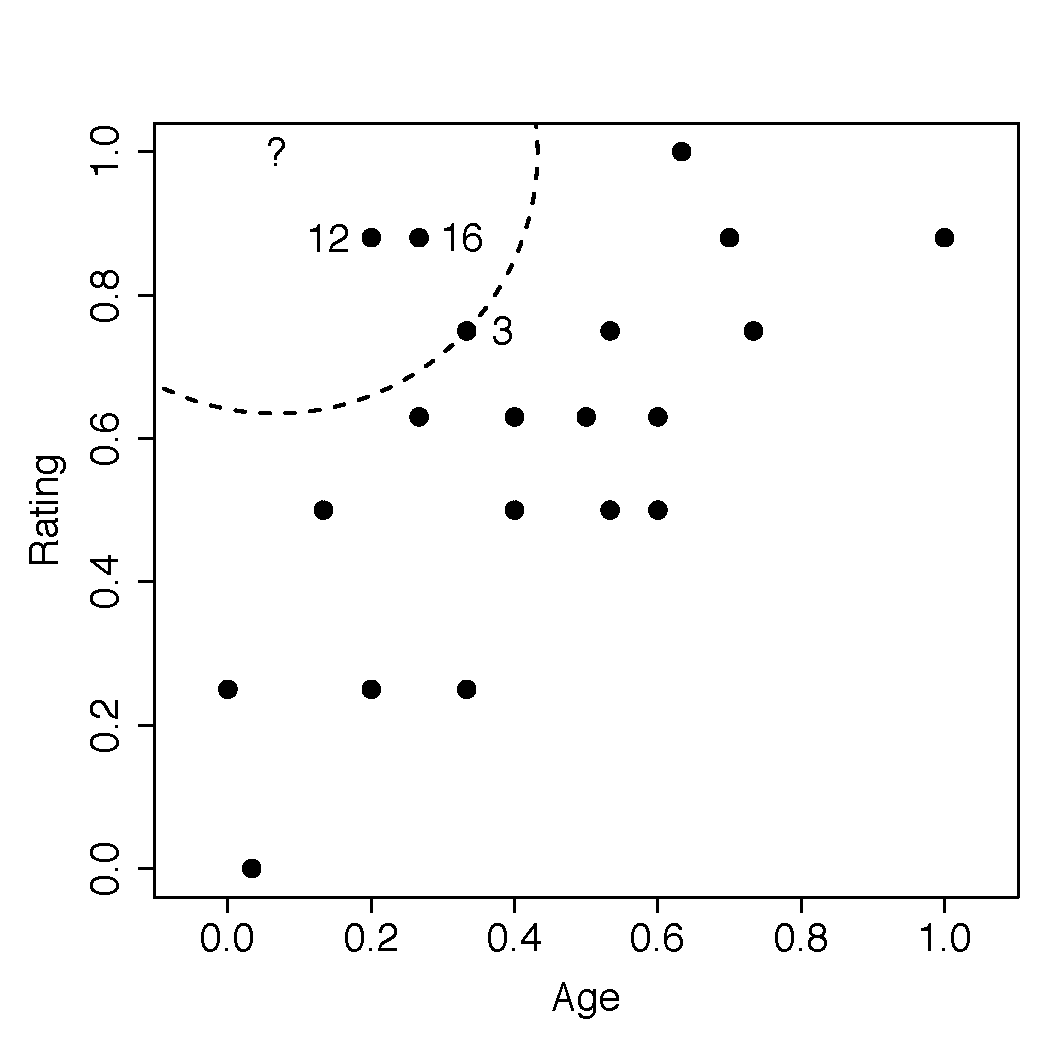
\includegraphics[width=0.62\textwidth]{./images/whiskey_fs.pdf}
	\end{center}
	\caption{The \featN{Age} and \featN{Rating} feature space for the whiskey dataset. The location of the query instance is indicated by the ? symbol. The circle plotted with a dashed line demarcates the border of the neighborhood around the query when $k=3$. The three nearest neighbors to the query are labelled with their \featN{ID} values.}
	\label{fig:whiskeyfs}
\end{figure}
\end{frame} 

 \begin{frame} 
 \begin{itemize}
\item The model will return a price prediction that is the average price of the three neighbors:
\begin{equation*}
\frac{200.00+250.00+55.00}{3}=168.33
\label{eq:whiskypricepred}
\end{equation*}
\end{itemize}
\end{frame} 


 \begin{frame} 
\begin{itemize}
	\item In a  \alert{weighted \textit{k} nearest neighbor} the model prediction equation is changed to:
\end{itemize}
\begin{equation}
\mathbb{M}_{k}(\mathbf{q}) =\frac{\displaystyle\sum_{i=1}^k \displaystyle \frac{1}{dist(\mathbf{q},\mathbf{d}_i)^2} \times t_i}{\displaystyle\sum_{i=1}^k \displaystyle \frac{1}{dist(\mathbf{q},\mathbf{d}_i)^2}} 
\label{eq:weightedknnreg}
\end{equation}
\end{frame} 



 \begin{frame}[plain]
\begin{table}[htb]
\caption{The calculations for the weighted \textit{k} nearest neighbor prediction}
\label{table:whiskeyPriceWeightedPred}
\begin{center}
\resizebox{\textheight}{!}{
\begin{Tiny}
\begin{tabular}[ht]{crrrrr} 
		\hline
\textbf{ID}	 & \textbf{Price} & \textbf{Distance} & \textbf{Weight} & \textbf{Price$\times$Weight}\\
\hline
1	&30.00	&0.7530	&1.7638	&52.92\\
2	&40.00	&0.5017	&3.9724	&158.90\\
3	&55.00	&0.3655	&7.4844	&411.64\\
4	&550.00	&0.6456	&2.3996	&1319.78\\
5	&35.00	&0.6009	&2.7692	&96.92\\
6	&45.00	&0.5731	&3.0450	&137.03\\
7	&70.00	&0.5294	&3.5679	&249.75\\
8	&85.00	&0.7311	&1.8711	&159.04\\
9	&78.00	&0.6520	&2.3526	&183.50\\
10	&75.00	&0.6839	&2.1378	&160.33\\
11	&500.00	&0.5667	&3.1142	&1557.09\\
12	&200.00	&0.1828	&29.9376	&5987.53\\
13	&65.00	&0.4250	&5.5363	&359.86\\
14	&120.00	&0.7120	&1.9726	&236.71\\
15	&12.00	&0.7618	&1.7233	&20.68\\
16	&250.00	&0.2358	&17.9775	&4494.38\\
17	&18.00	&0.7960	&1.5783	&28.41\\
18	&450.00	&0.9417	&1.1277	&507.48\\
19	&10.00	&1.0006	&0.9989	&9.99\\
20	&30.00	&0.5044	&3.9301	&117.90\\
\hline
\multicolumn{3}{r}{\textbf{Totals:}} & 99.2604 & 16\,249.85\\ 
				\end{tabular}
\end{Tiny}
}
\end{center}
\end{table}
\end{frame} 

\SectionSlideShortHeader{Other Measures of Similarity}{Similarity}



 \begin{frame} 
\begin{table}[!tb]
\caption{A binary dataset listing the behavior of two individuals on a website during a trial period and whether or not they subsequently signed-up for the website.}
\label{table:binaryDataset}
\centering
\begin{footnotesize}
\begin{tabular}{  c  c  c  c  c  c  c }
\hline
\textbf{ID} & \textbf{Profile} & \textbf{FAQ} & \textbf{Help Forum} & \textbf{Newsletter} & \textbf{Liked} & \textbf{Signup}\\
\hline
1  &  1 & 1 & 1 & 0 & 1 & Yes\\
2  &  1 & 0 & 0 & 0 & 0 & No\\
\hline
\end{tabular}
\end{footnotesize}
\end{table}
\end{frame} 

\begin{frame}
\begin{alertblock}{Who is $\mathbf{q}$ more similar to $\mathbf{d}_1$ or $\mathbf{d}_2$?}
\begin{footnotesize}
\begin{equation*}
\mathbf{q} =  \left< \text{\featN{Profile}:}1, \text{\featN{FAQ}:}0, \text{\featN{Help Forum}:}1, \text{\featN{Newsletter}:}0, \text{\featN{Liked}:}0,\right>  
\end{equation*}
\end{footnotesize}

~\\

\resizebox{\textwidth}{!}{\begin{tabular}{  c  c  c  c  c  c  c }
\hline
\textbf{ID} & \textbf{Profile} & \textbf{FAQ} & \textbf{Help Forum} & \textbf{Newsletter} & \textbf{Liked} & \textbf{Signup}\\
\hline
1  &  1 & 1 & 1 & 0 & 1 & Yes\\
2  &  1 & 0 & 0 & 0 & 0 & No\\
\hline
\end{tabular}
}
\end{alertblock}
\end{frame}

 \begin{frame} 
\begin{table}[htb]
	\begin{tabular}{cc}
		\begin{minipage}[t]{0.49\textwidth}
			\centerline{
				\begin{tabular} {cc|cc}
				~ & ~ 	& \multicolumn{2}{c}{$\mathbf{q}$}\\
				~ & ~	 & Pres. & Abs.\\
				\hline
				\multirow{2}{*}{$\mathbf{d}_1$}& Pres. & CP=2 & PA=0\\
				& Abs. & AP=2 & CA=1\\
				\end{tabular}
			}
		\end{minipage}
		&
		\hfill \begin{minipage}[t]{0.49\textwidth}
			\centerline{
				\begin{tabular} {cc|cc}
				~ & ~ 	& \multicolumn{2}{c}{$\mathbf{q}$}\\
				~ & ~	 & Pres. & Abs.\\
				\hline
				\multirow{2}{*}{$\mathbf{d}_2$}& Pres. & CP=1 & PA=1\\
				& Abs. & AP=0 & CA=3\\
				\end{tabular}
			}
		\end{minipage}
	\end{tabular}
			\caption{The similarity between the current trial user, $\mathbf{q}$, and the two users in the dataset, $\mathbf{d}_1$ and $\mathbf{d}_2$, in terms of co-presence (CP), co-absence (CA), presence-absence (PA), and absence-presence (AP).}
			\label{table:binaryDatasetAnalysis}
\end{table}
\end{frame} 




 \begin{frame} 
\begin{block}{Russel-Rao}
\begin{itemize}
	\item The ratio between the number of co-presenses and the total number of binary features considered.
\end{itemize}
\begin{equation}
sim_{RR}(\mathbf{q},\mathbf{d})=\frac{CP(\mathbf{q},\mathbf{d})}{|\mathbf{q}|}
\label{eq:russel-rao}
\end{equation}
\end{block}
\end{frame} 

 \begin{frame} 
\begin{block}{Russel-Rao}
\begin{equation}
sim_{RR}(\mathbf{q},\mathbf{d})=\frac{CP(\mathbf{q},\mathbf{d})}{|\mathbf{q}|}
\label{eq:russel-rao}
\end{equation}
\end{block}
\begin{equation*}
 \left< \text{\featN{Profile}:}1, \text{\featN{FAQ}:}0, \text{\featN{Help Forum}:}1, \text{\featN{Newsletter}:}0, \text{\featN{Liked}:}0,\right>  
\end{equation*}
	\begin{tabular}{cc}
		\begin{minipage}[t]{0.49\textwidth}
			\centerline{
				\begin{tabular} {cc|cc}
				~ & ~ 	& \multicolumn{2}{c}{$\mathbf{q}$}\\
				~ & ~	 & Pres. & Abs.\\
				\hline
				\multirow{2}{*}{$\mathbf{d}_1$}& Pres. & CP=2 & PA=0\\
				& Abs. & AP=2 & CA=1\\
				\end{tabular}
			}
		\end{minipage}
		&
		\hfill \begin{minipage}[t]{0.49\textwidth}
			\centerline{
				\begin{tabular} {cc|cc}
				~ & ~ 	& \multicolumn{2}{c}{$\mathbf{q}$}\\
				~ & ~	 & Pres. & Abs.\\
				\hline
				\multirow{2}{*}{$\mathbf{d}_2$}& Pres. & CP=1 & PA=1\\
				& Abs. & AP=0 & CA=3\\
				\end{tabular}
			}
		\end{minipage}
	\end{tabular}
\end{frame} 



 \begin{frame} 
\begin{block}{Russel-Rao}
\begin{equation}
sim_{RR}(\mathbf{q},\mathbf{d})=\frac{CP(\mathbf{q},\mathbf{d})}{|\mathbf{q}|}
\label{eq:russel-rao}
\end{equation}
\end{block}
\begin{example}
\begin{eqnarray*}
sim_{RR}(\mathbf{q},\mathbf{d}_1)=\frac{2}{5}=0.4\\
sim_{RR}(\mathbf{q},\mathbf{d}_2)=\frac{1}{5}=0.2\\
\end{eqnarray*}
\begin{itemize}
	\item The current trial user is judged to be more similar to instance $\mathbf{d}_1$ then $\mathbf{d}_2$.
\end{itemize}
\end{example}
\end{frame} 

 \begin{frame} 
\begin{block}{Sokal-Michener}
\begin{itemize}
	\item Sokal-Michener is defined as the ratio between the total number of co-presences and co-absences, and the total number of binary features considered.
\end{itemize}
\begin{equation}
sim_{SM}(\mathbf{q},\mathbf{d})=\frac{CP(\mathbf{q},\mathbf{d})+CA(\mathbf{q},\mathbf{d})}{|\mathbf{q}|}
\label{eq:sokal-michener}
\end{equation}
\end{block}
\end{frame} 

 \begin{frame} 
\begin{block}{Sokal-Michener}
\begin{equation}
sim_{SM}(\mathbf{q},\mathbf{d})=\frac{CP(\mathbf{q},\mathbf{d})+CA(\mathbf{q},\mathbf{d})}{|\mathbf{q}|}
\label{eq:sokal-michener}
\end{equation}
\end{block}
\begin{equation*}
 \left< \text{\featN{Profile}:}1, \text{\featN{FAQ}:}0, \text{\featN{Help Forum}:}1, \text{\featN{Newsletter}:}0, \text{\featN{Liked}:}0,\right>  
\end{equation*}
	\begin{tabular}{cc}
		\begin{minipage}[t]{0.49\textwidth}
			\centerline{
				\begin{tabular} {cc|cc}
				~ & ~ 	& \multicolumn{2}{c}{$\mathbf{q}$}\\
				~ & ~	 & Pres. & Abs.\\
				\hline
				\multirow{2}{*}{$\mathbf{d}_1$}& Pres. & CP=2 & PA=0\\
				& Abs. & AP=2 & CA=1\\
				\end{tabular}
			}
		\end{minipage}
		&
		\hfill \begin{minipage}[t]{0.49\textwidth}
			\centerline{
				\begin{tabular} {cc|cc}
				~ & ~ 	& \multicolumn{2}{c}{$\mathbf{q}$}\\
				~ & ~	 & Pres. & Abs.\\
				\hline
				\multirow{2}{*}{$\mathbf{d}_2$}& Pres. & CP=1 & PA=1\\
				& Abs. & AP=0 & CA=3\\
				\end{tabular}
			}
		\end{minipage}
	\end{tabular}
\end{frame} 

 \begin{frame} 
\begin{block}{Sokal-Michener}
\begin{equation}
sim_{SM}(\mathbf{q},\mathbf{d})=\frac{CP(\mathbf{q},\mathbf{d})+CA(\mathbf{q},\mathbf{d})}{|\mathbf{q}|}
\label{eq:sokal-michener}
\end{equation}
\end{block}
\begin{example}
\begin{eqnarray*}
sim_{SM}(\mathbf{q},\mathbf{d}_1)=\frac{3}{5}=0.6\\
sim_{SM}(\mathbf{q},\mathbf{d}_2)=\frac{4}{5}=0.8\\
\end{eqnarray*}
\begin{itemize}
	\item The current trial user is judged to be more similar to instance $\mathbf{d}_2$ then $\mathbf{d}_1$.
\end{itemize}
\end{example}
\end{frame} 



 \begin{frame} 
\begin{block}{Jaccard}
\begin{itemize}
	\item The Jacquard index ignore co-absences
\end{itemize}
\begin{equation}
sim_{J}(\mathbf{q},\mathbf{d})=\frac{CP(\mathbf{q},\mathbf{d})}{CP(\mathbf{q},\mathbf{d})+PA(\mathbf{q},\mathbf{d})+AP(\mathbf{q},\mathbf{d})}
\label{eq:jaccard}
\end{equation}
\end{block}
\end{frame} 

 \begin{frame} 
\begin{block}{Jaccard}
\begin{equation}
sim_{J}(\mathbf{q},\mathbf{d})=\frac{CP(\mathbf{q},\mathbf{d})}{CP(\mathbf{q},\mathbf{d})+PA(\mathbf{q},\mathbf{d})+AP(\mathbf{q},\mathbf{d})}
\label{eq:jaccard}
\end{equation}
\end{block}
\begin{equation*}
 \left< \text{\featN{Profile}:}1, \text{\featN{FAQ}:}0, \text{\featN{Help Forum}:}1, \text{\featN{Newsletter}:}0, \text{\featN{Liked}:}0,\right>  
\end{equation*}
	\begin{tabular}{cc}
		\begin{minipage}[t]{0.49\textwidth}
			\centerline{
				\begin{tabular} {cc|cc}
				~ & ~ 	& \multicolumn{2}{c}{$\mathbf{q}$}\\
				~ & ~	 & Pres. & Abs.\\
				\hline
				\multirow{2}{*}{$\mathbf{d}_1$}& Pres. & CP=2 & PA=0\\
				& Abs. & AP=2 & CA=1\\
				\end{tabular}
			}
		\end{minipage}
		&
		\hfill \begin{minipage}[t]{0.49\textwidth}
			\centerline{
				\begin{tabular} {cc|cc}
				~ & ~ 	& \multicolumn{2}{c}{$\mathbf{q}$}\\
				~ & ~	 & Pres. & Abs.\\
				\hline
				\multirow{2}{*}{$\mathbf{d}_2$}& Pres. & CP=1 & PA=1\\
				& Abs. & AP=0 & CA=3\\
				\end{tabular}
			}
		\end{minipage}
	\end{tabular}
\end{frame} 

 \begin{frame} 
\begin{block}{Jaccard}
\begin{equation}
sim_{J}(\mathbf{q},\mathbf{d})=\frac{CP(\mathbf{q},\mathbf{d})}{CP(\mathbf{q},\mathbf{d})+PA(\mathbf{q},\mathbf{d})+AP(\mathbf{q},\mathbf{d})}
\label{eq:jaccard}
\end{equation}
\end{block}
\begin{example}
\begin{eqnarray*}
sim_{J}(\mathbf{q},\mathbf{d}_1)=\frac{2}{4}=0.5\\
sim_{J}(\mathbf{q},\mathbf{d}_2)=\frac{1}{2}=0.5\\
\end{eqnarray*}
\begin{itemize}
	\item The current trial user is judged to be equally similar to instance $\mathbf{d}_1$ and $\mathbf{d}_2$!
\end{itemize}
\end{example}
\end{frame} 





\begin{frame}
	\begin{itemize}
	\item \alert{Cosine similarity} between two instances is the cosine of the inner angle between the two vectors that extend from the origin to each instance.
	\end{itemize}
\begin{block}{Cosine}
\begin{equation*}
sim_{COSINE}(\mathbf{a}, \mathbf{b}) = \frac{\left(\mathbf{a}[1] \times \mathbf{b}[1] \right)+ \dots + \left(\mathbf{a}[m] \times \mathbf{b}[m]\right)}{\sqrt{\sum_{i=1}^m \mathbf{a}[i]^2} \times \sqrt{\sum_{i=1}^m \mathbf{b}[i]^2}}
\label{eq:cosinesim}
\end{equation*}
\end{block}
\end{frame}


 \begin{frame} 
 \begin{itemize}
	\item Calculate the cosine similarity between the following two instances:
\end{itemize}
\begin{equation*}
	 \mathbf{d}_{1} = \< \featN{SMS} = 97, \featN{Voice} = 21 \>
\end{equation*}
\begin{equation*}
	 \mathbf{d}_{2} = \< \featN{SMS} = 18,  \featN{Voice} = 184 \>
\end{equation*}
\begin{equation*}
sim_{COSINE}(\mathbf{a}, \mathbf{b}) =  \displaystyle\frac{\sum_{i=1}^m \left(\mathbf{a}[i] \times \mathbf{b}[i]\right) }{\sqrt{\sum_{i=1}^m \mathbf{a}[i]^2} \times \sqrt{\sum_{i=1}^m \mathbf{b}[i]^2}}
\end{equation*}
\end{frame} 



 \begin{frame} 
 \begin{itemize}
	\item Calculate the cosine similarity between the following two instances:
\end{itemize}
\begin{equation*}
	 \mathbf{d}_{1} = \< \featN{SMS} = 97, \featN{Voice} = 21 \>
\end{equation*}
\begin{equation*}
	 \mathbf{d}_{2} = \< \featN{SMS} = 18,  \featN{Voice} = 184 \>
\end{equation*}
\begin{equation*}
	\begin{alignedat}{2}
sim_{COSINE}(\mathbf{d}_{1}, \mathbf{d}_{1}) &= \frac{\left(97 \times 181 \right)+ \left(21 \times 184\right)}{\sqrt{97^2 + 21^2} \times \sqrt{181^2 + 184^2}}\\
&= 0.8362
	\end{alignedat}
\end{equation*}
\end{frame} 



 \begin{frame} 
\begin{figure}[htb]
	\begin{centering}
		\subfigure[]{\label{fig:cosine}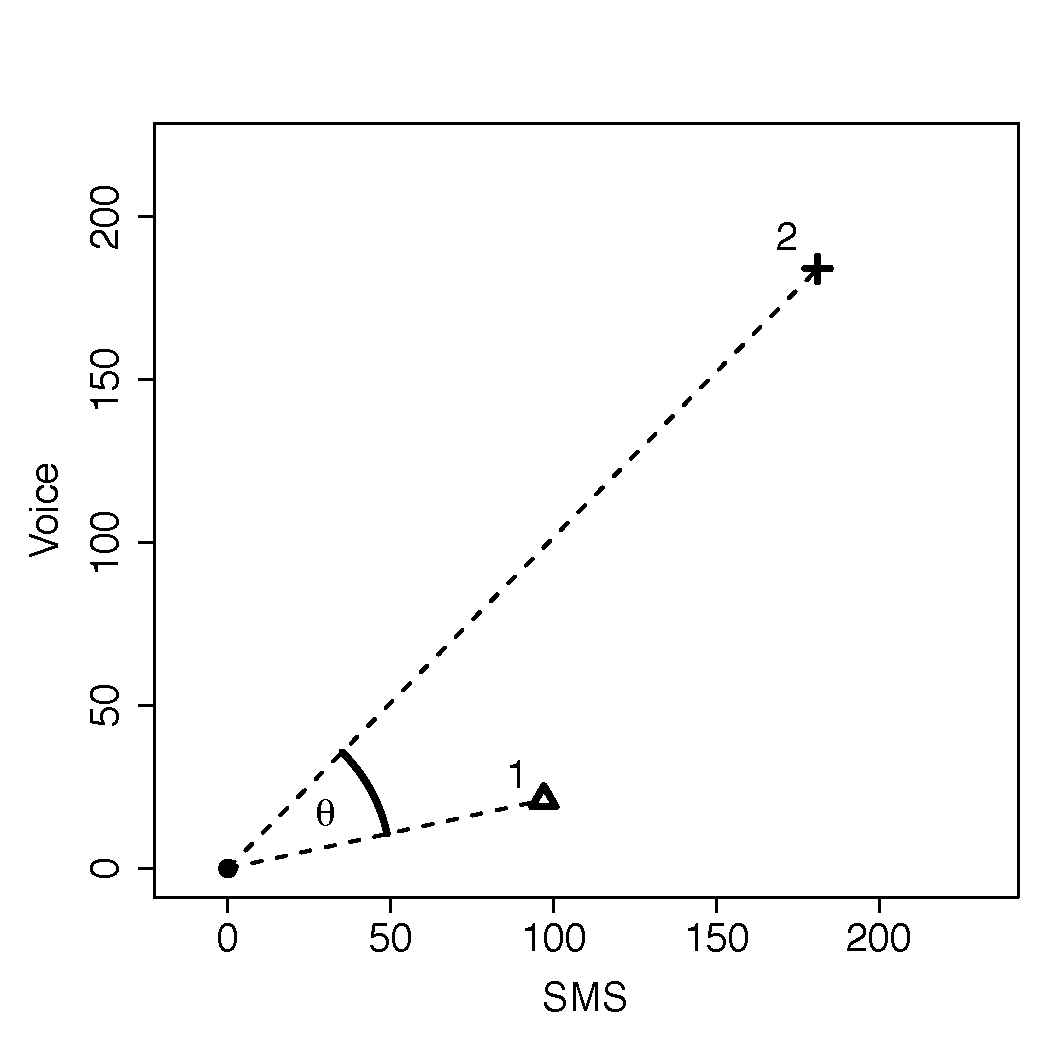
\includegraphics[width=0.45\textwidth]{./images/cosine1.pdf}}
		\subfigure[]{\label{fig:cosineNorm}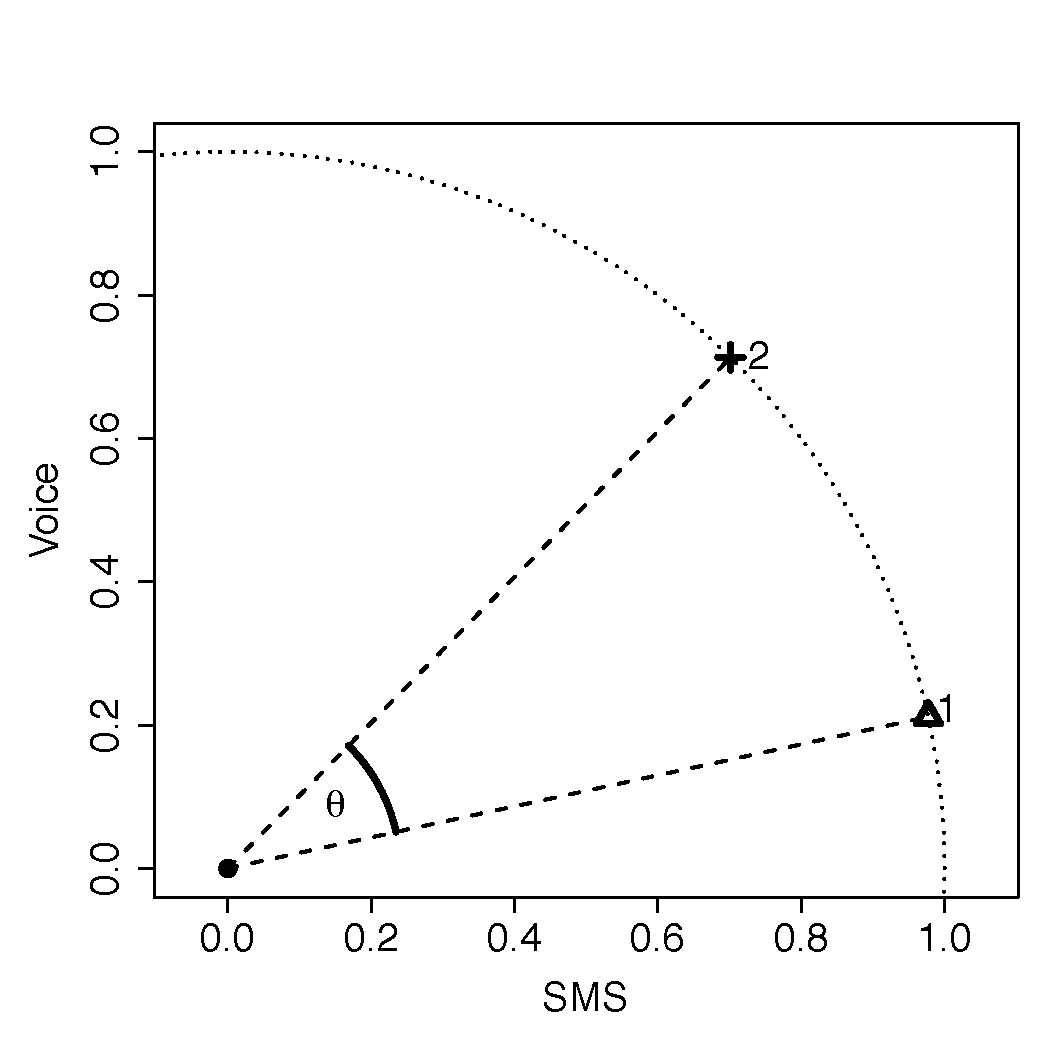
\includegraphics[width=0.45\textwidth]{./images/cosine2.pdf}}
	\caption{(a) The $\theta$ represents the inner angle between the vector emanating from the origin to instance $\mathbf{d}_{1}$ $\left<\featN{SMS}= 97, \featN{Voice}=21 \right>$ and the vector emanating from the origin to instance $\mathbf{d}_{2}$ $\left< \featN{SMS}=181, \featN{Voice}=184\right>$; (b) shows $\mathbf{d}_{1}$ and $\mathbf{d}_{2}$ normalized to the unit circle.}
	\label{fig:cosineImages}
		\end{centering}
\end{figure}
\end{frame} 

 \begin{frame} 
 \begin{itemize}
	\item Calculate the cosine similarity between the following two instances:
\end{itemize}
\begin{equation*}
	 \mathbf{d}_{1} = \< \featN{SMS} = 97, \featN{Voice} = 21 \>
\end{equation*}
\begin{equation*}
	 \mathbf{d}_{3} = \< \featN{SMS} = 194,  \featN{Voice} = 42 \>
\end{equation*}
\begin{equation*}
sim_{COSINE}(\mathbf{a}, \mathbf{b}) =  \displaystyle\frac{\sum_{i=1}^m \left(\mathbf{a}[i] \times \mathbf{b}[i]\right) }{\sqrt{\sum_{i=1}^m \mathbf{a}[i]^2} \times \sqrt{\sum_{i=1}^m \mathbf{b}[i]^2}}
\end{equation*}
\end{frame} 

 \begin{frame} 
 \begin{itemize}
	\item Calculate the cosine similarity between the following two instances:
\end{itemize}
\begin{equation*}
	 \mathbf{d}_{1} = \< \featN{SMS} = 97, \featN{Voice} = 21 \>
\end{equation*}
\begin{equation*}
	 \mathbf{d}_{3} = \< \featN{SMS} = 194,  \featN{Voice} = 42 \>
\end{equation*}
\begin{equation*}
	\begin{alignedat}{2}
sim_{COSINE}(\mathbf{d}_{1}, \mathbf{d}_{1}) &= \frac{\left(97 \times 194 \right)+ \left(21 \times 42\right)}{\sqrt{97^2 + 21^2} \times \sqrt{194^2 + 42^2}}\\
&= \alert{1}
	\end{alignedat}
\end{equation*}
\end{frame} 

 \begin{frame} 
\begin{figure}[htb]
	\begin{center}
\begin{tabular}{ccc}
\subfigure[]{\label{fig:mahalanobis1}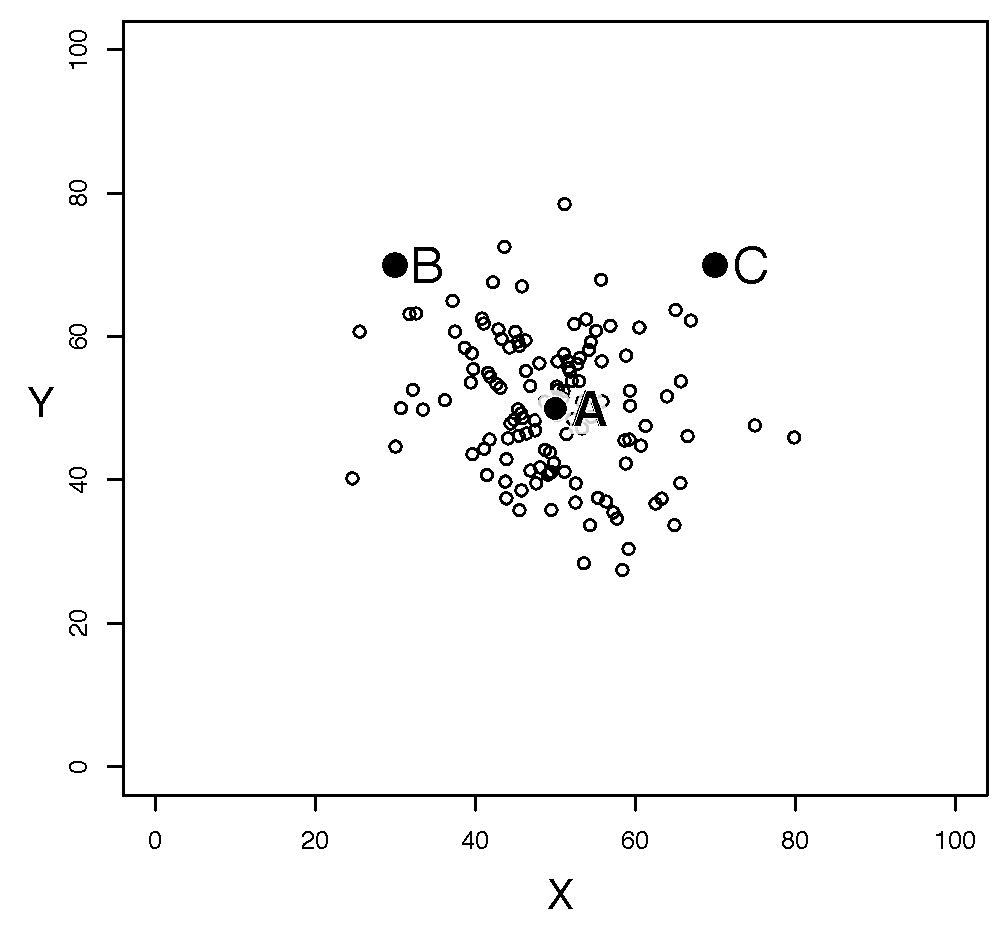
\includegraphics[width=0.32\textwidth]{./images/mahalanobis_1_A.pdf}}&
\subfigure[]{\label{fig:mahalanobis2}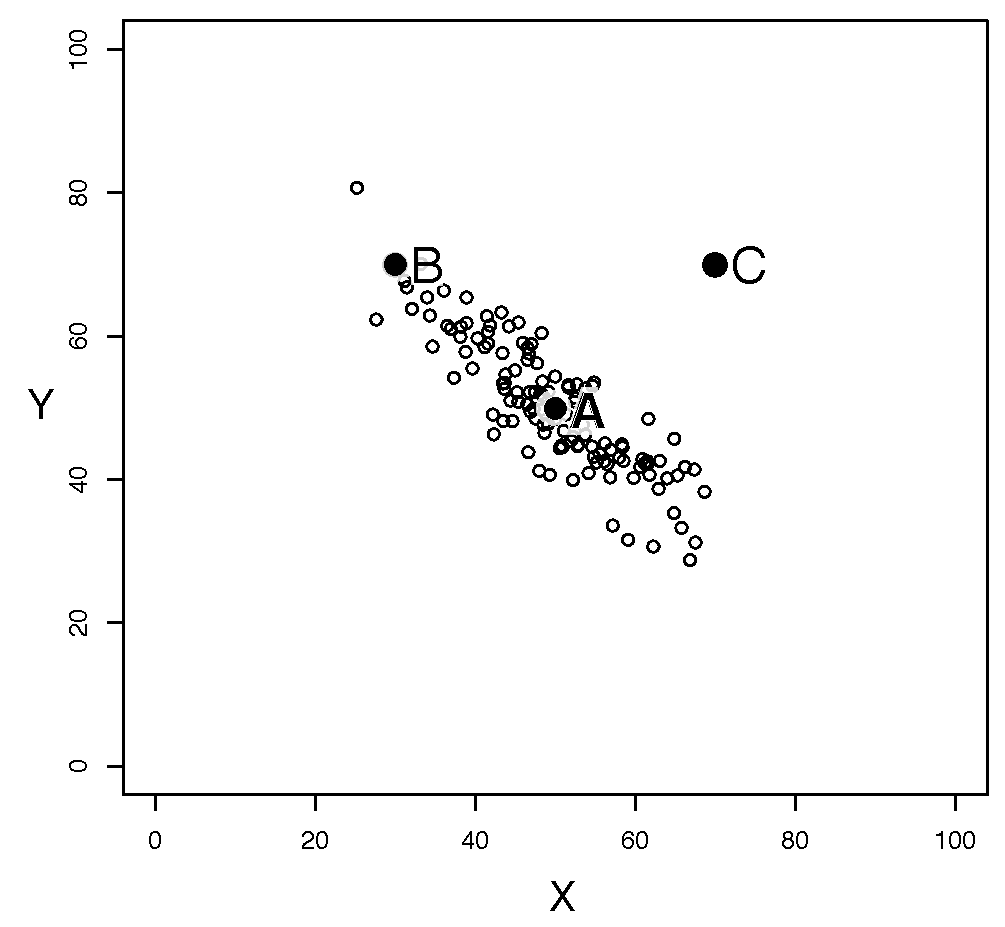
\includegraphics[width=0.32\textwidth]{./images/mahalanobis_2_A.pdf}}&		
\subfigure[]{\label{fig:mahalanobis3}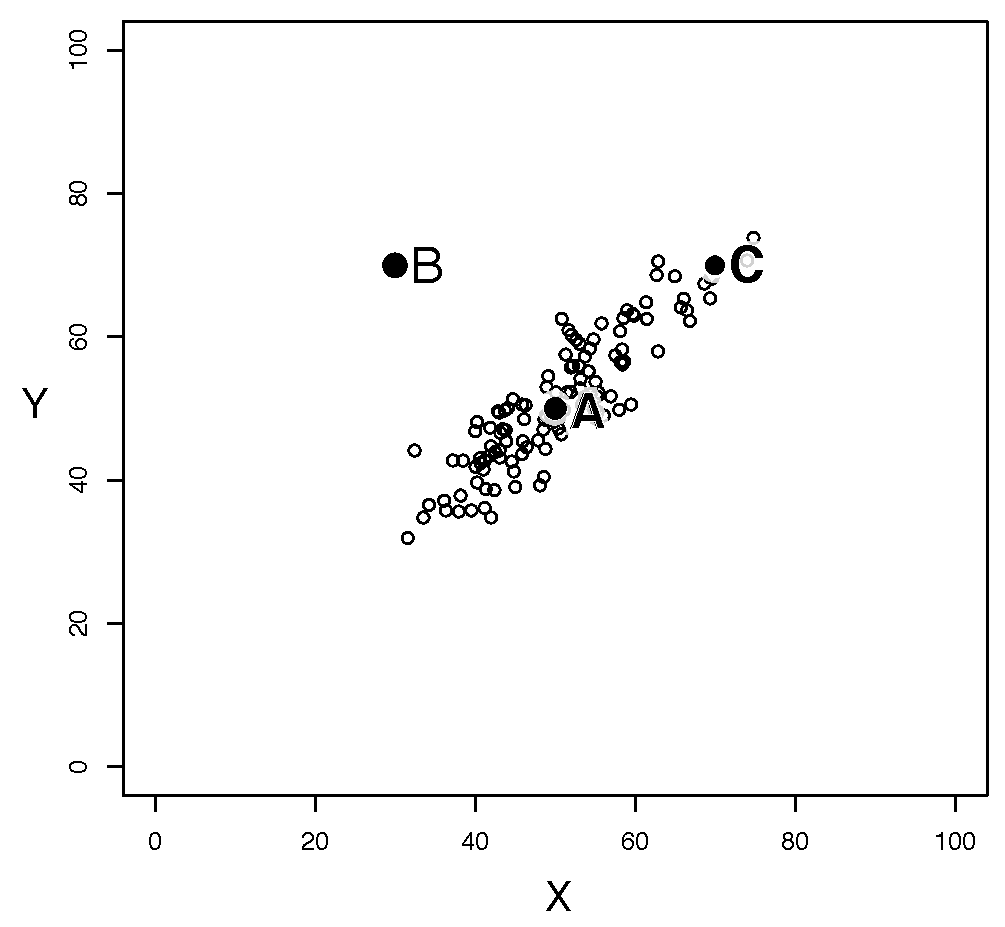
\includegraphics[width=0.32\textwidth]{./images/mahalanobis_3_A.pdf}}
	\end{tabular}
	\end{center}
       \caption{Scatter plots of three bivariate datasets with the same center point A and two queries B and C both equidistant from A. (a) A dataset uniformly spread around the center point. (b) A dataset with negative covariance. (c) A dataset with positive covariance.}  
	\label{fig:mahalanobis_motivation}
\end{figure}
\end{frame} 

\begin{frame}
	\begin{itemize}
		\item The mahalanobis distance uses covariance to scale distances so that distances along a direction where the dataset is spreadout a lot are scaled down and distances along directions where the dataset is tightly packed are scaled up. 
	\end{itemize}
\begin{equation}
	\begin{alignedat}{2}
&Mahalanobis(\mathbf{a},\mathbf{b}) =\\
&\left[\mathbf{a}[1] - \mathbf{b}[1], \ldots, \mathbf{a}[m] - \mathbf{b}[m] \right] \times \sum^{-1} \times    \left[   \begin{matrix} \mathbf{a}[1] - \mathbf{b}[1]\\ \ldots \\ \mathbf{a}[m] - \mathbf{b}[m] \end{matrix} \right]
	\end{alignedat}
\label{eq:mahalanobis}
\end{equation}
\end{frame} 


\begin{frame}
	\begin{itemize}
		\item Similar to Euclidean distance, the mahalanobis distance squares the differences of the features. 
		\item But it also rescales the differences (using the inverse covariance matrix) so that all the features have unit variance and the effects of covariance is removed. 
	\end{itemize}
\end{frame} 

 \begin{frame} 
\begin{figure}[htb]
	\begin{center}
\begin{tabular}{ccc}
\subfigure[]{\label{fig:mahalanobis4}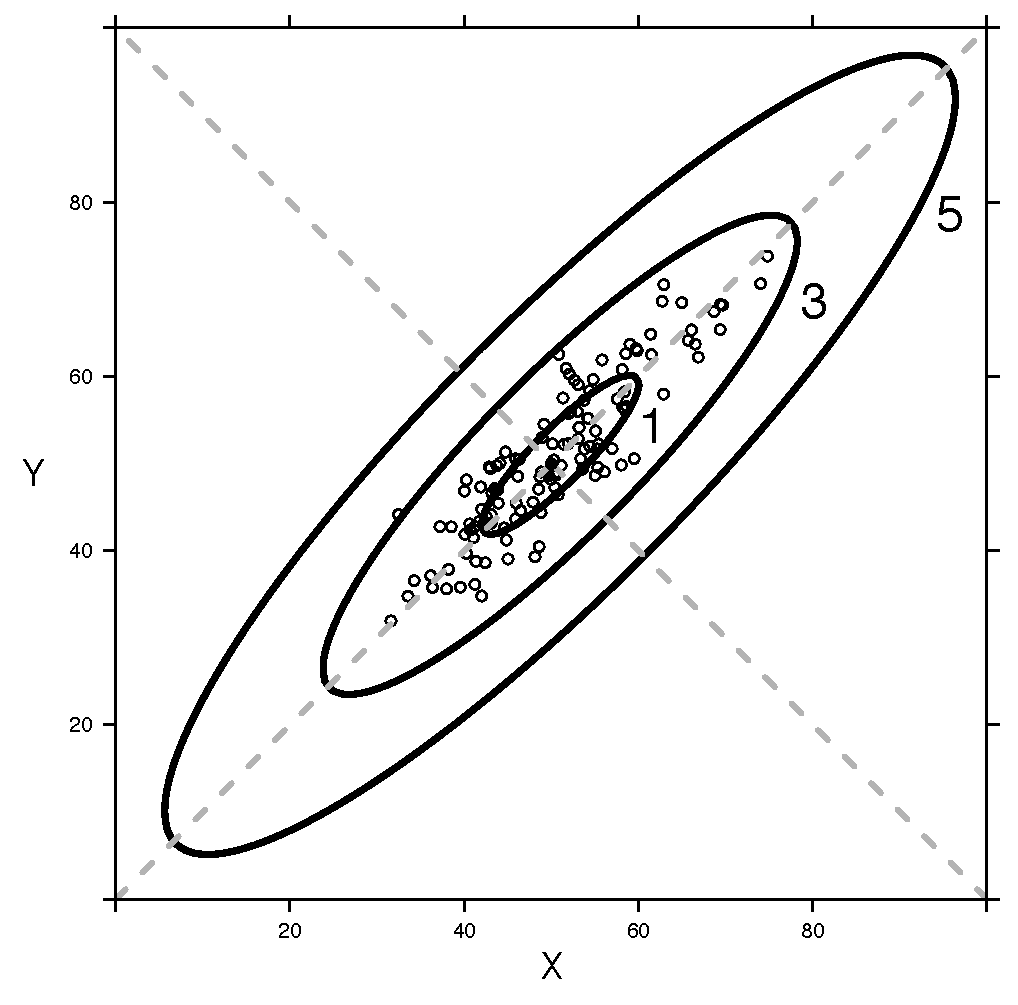
\includegraphics[width=0.32\textwidth]{./images/mahalanobis_4_A.pdf}}&
\subfigure[]{\label{fig:mahalanobis5}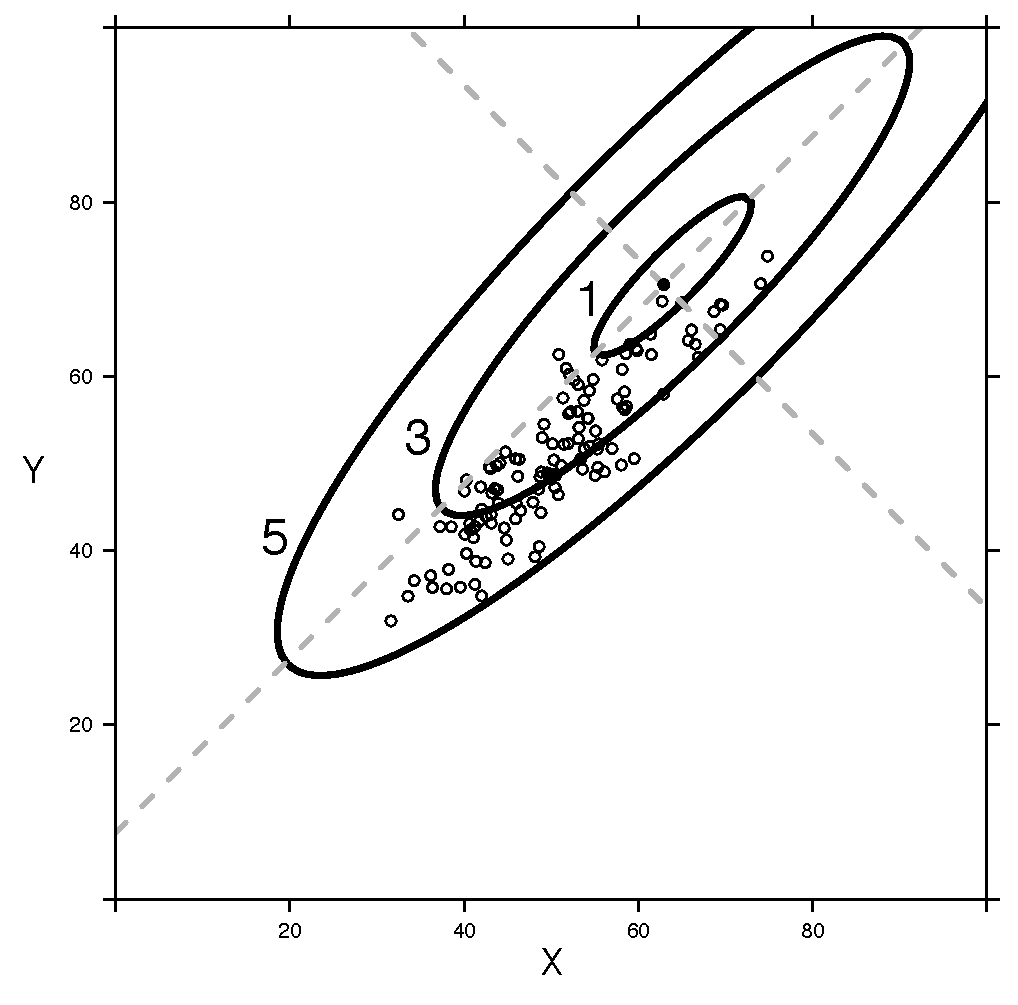
\includegraphics[width=0.32\textwidth]{./images/mahalanobis_5_A.pdf}}&		
\subfigure[]{\label{fig:mahalanobis6}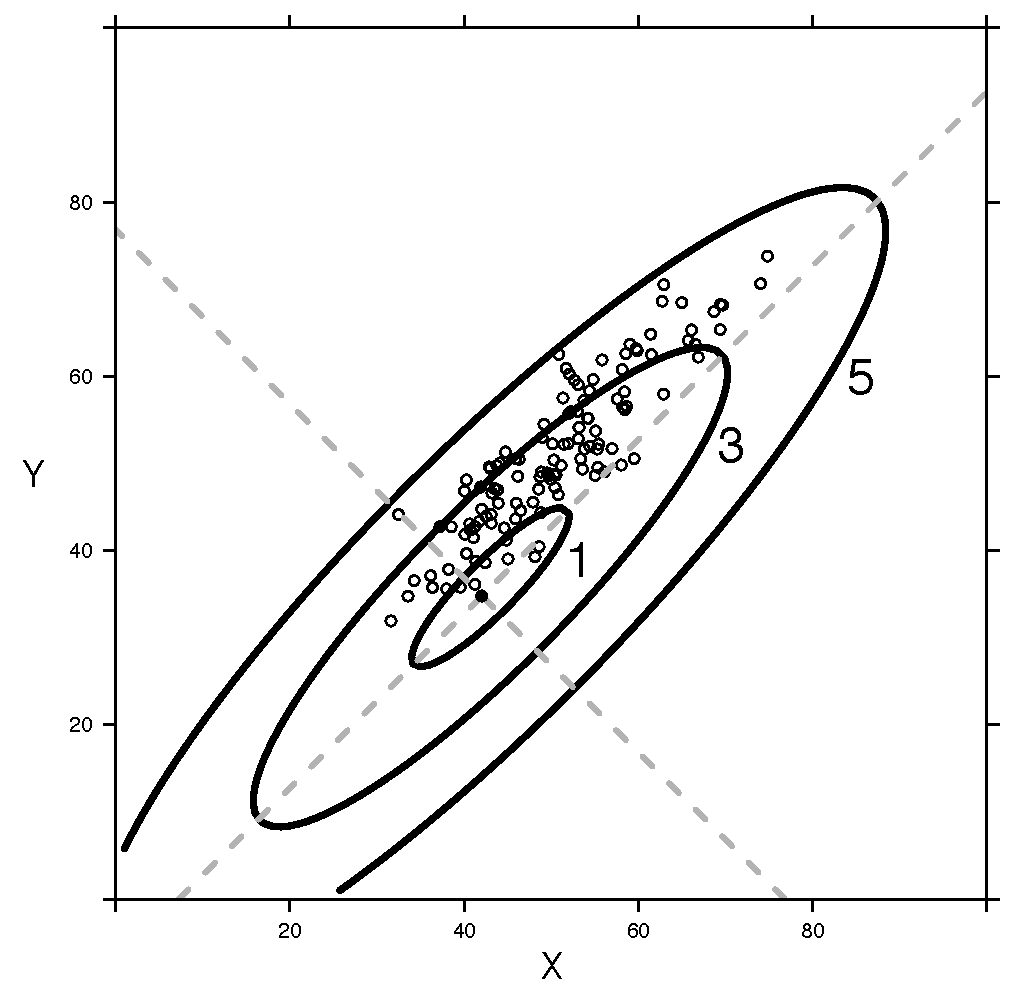
\includegraphics[width=0.32\textwidth]{./images/mahalanobis_6_A.pdf}}
	\end{tabular}
	\end{center}
       \caption{The coordinate systems defined by the mahalanobis metric using the co-variance matrix for the dataset in Figure \ourRef{fig:mahalanobis3} using three different origins: (a) $(50,50)$, (b) $(63,71)$, (c) $(42,35)$. The ellipses in each figure plot the $1$, $3$, and $5$ unit distances contours from each origin.}
	\label{fig:mahalanobis}
\end{figure}
\end{frame} 

 \begin{frame} 
\begin{figure}[htb]
       \begin{centering}
       \includegraphics[width=0.5\textwidth]{images/mahalanobis_7.pdf}
       \caption{The effect of using a mahalanobis versus euclidean distance. Point A is the center of mass of the dataset in Figure \ourRef{fig:mahalanobis3}. The ellipses plot the mahalanobis distance contours from A that B and C lie on. In euclidean terms B and C are equidistant from A, however using the mahalanobis metric C is much closer to A than B.}
       \label{fig:mahalanobis_euclidean}
       \end{centering}
\end{figure}
\end{frame} 

\SectionSlideShortHeader{Feature Selection}{Feat. Sel.}

\begin{frame} 
\begin{figure}
\begin{tabular}{ccc}
\subfigure[]{\label{fig:curse1d}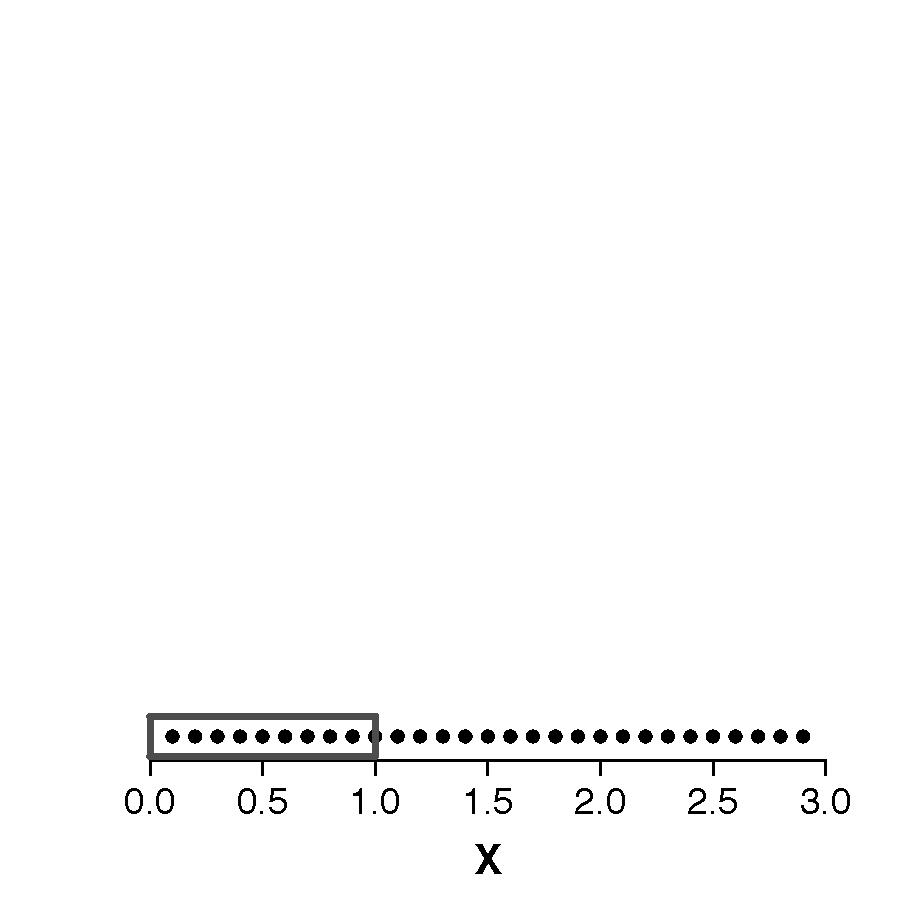
\includegraphics[width=0.32\textwidth]{./images/curse1D_BW.pdf}}&
\subfigure[]{\label{fig:curse2Dsparse}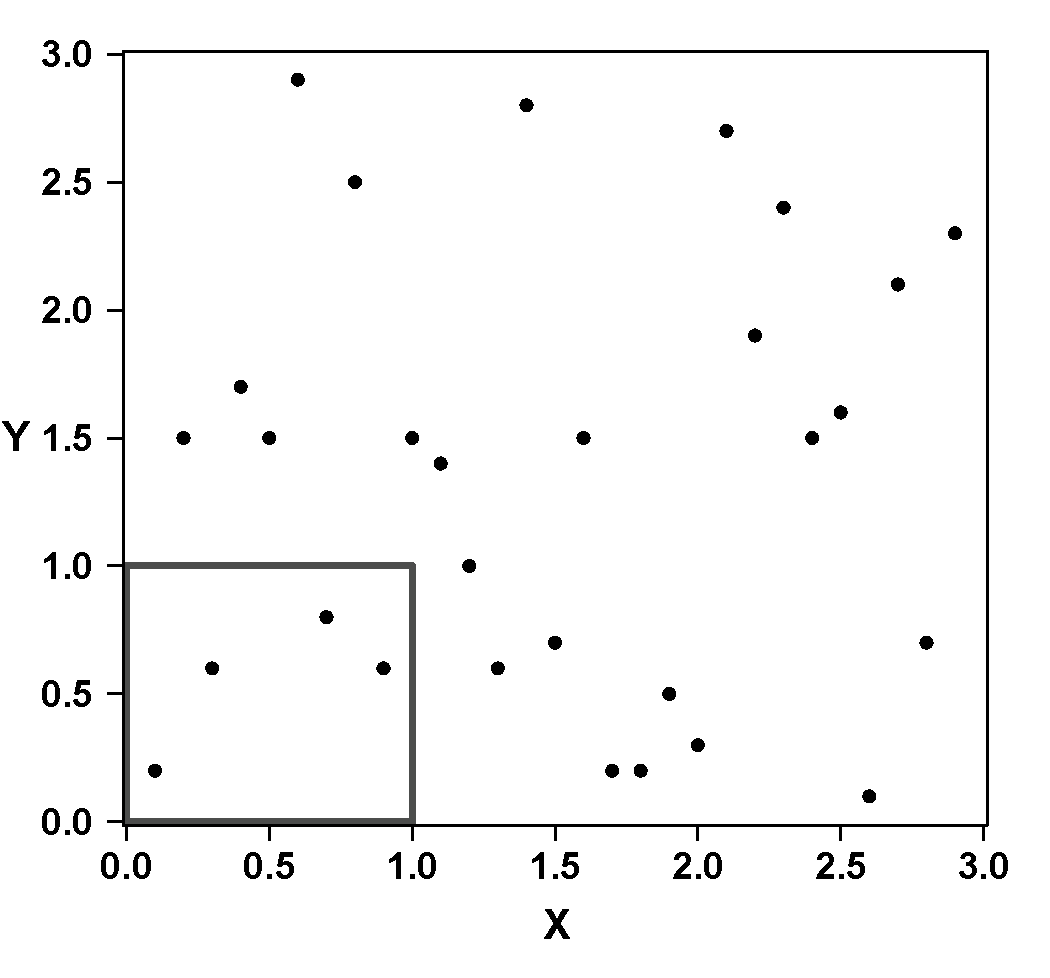
\includegraphics[width=0.32\textwidth]{./images/curse2Dsparse_BW.pdf}}&
\subfigure[]{\label{fig:curse3Dsparse}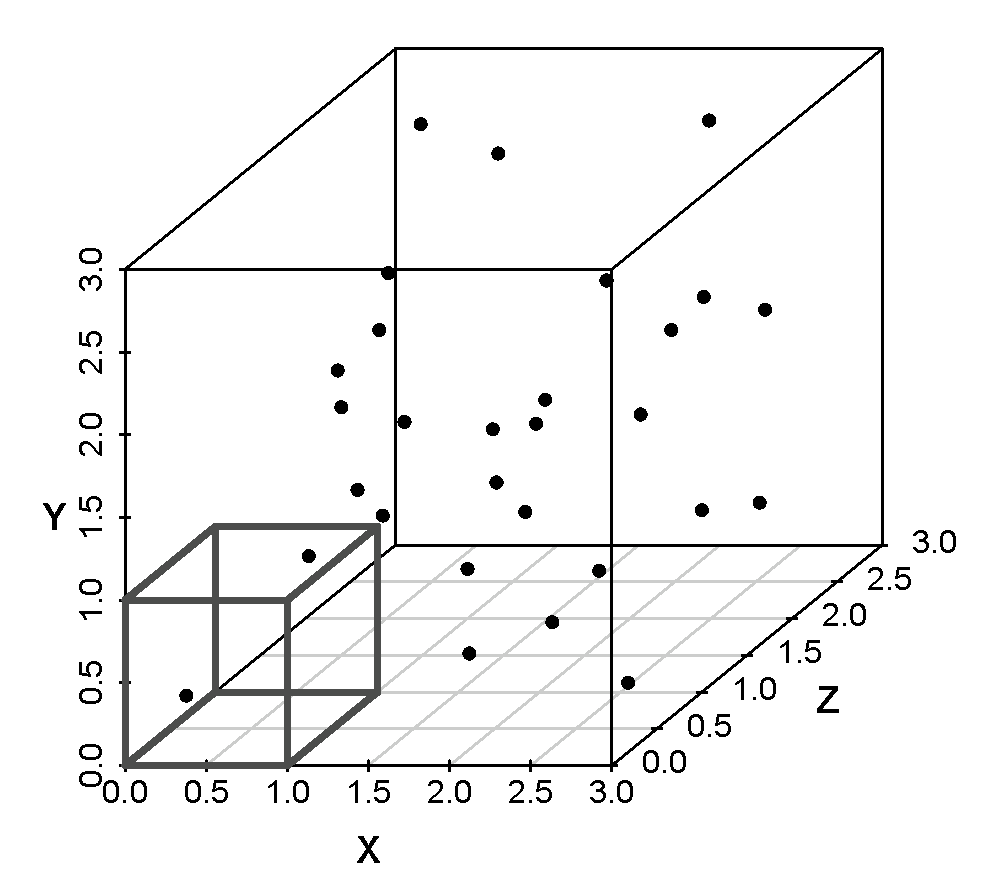
\includegraphics[width=0.32\textwidth]{./images/curse3Dsparse_BW.pdf}}
\end{tabular}
\caption{A set of scatter plots illustrating the curse of dimensionality. Across figures (a), (b) and (c) the density of the marked unit hypercubes decreases as the number of dimensions increases.}
\label{fig:curseofdimen}
\end{figure}
\end{frame} 

 \begin{frame} [plain]
\begin{figure}
\begin{tabular}{ccc}
\subfigure[]{\label{fig:curse1d}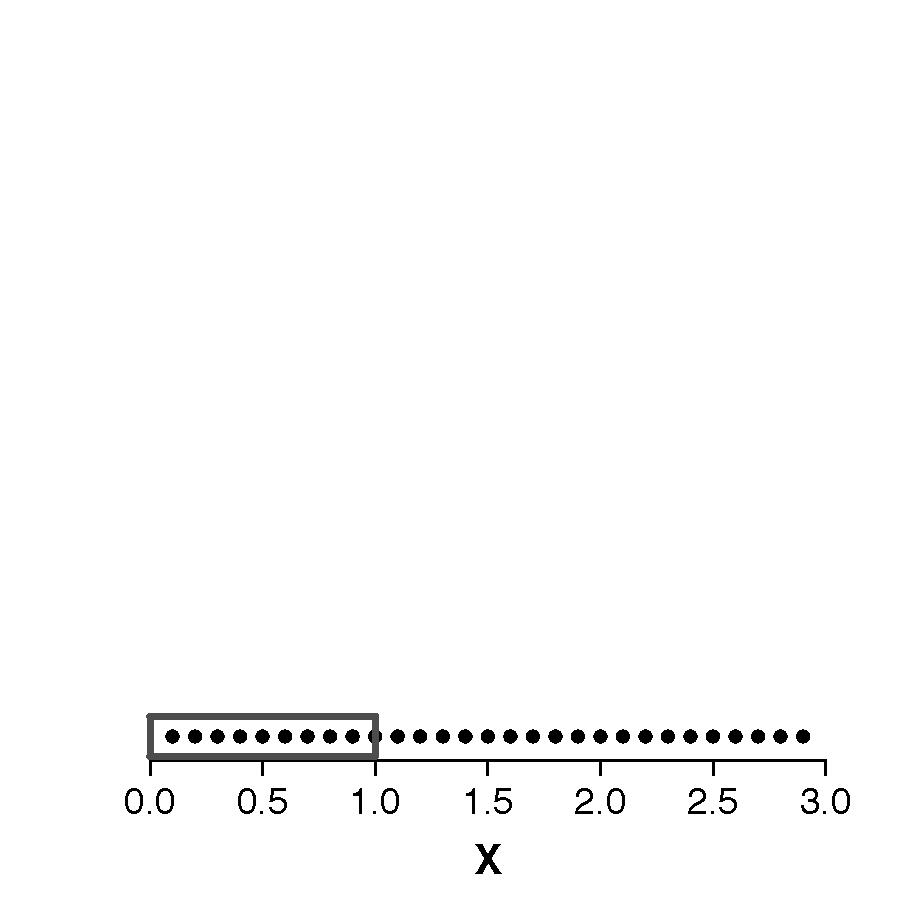
\includegraphics[width=0.28\textwidth]{./images/curse1D_BW.pdf}}&
\subfigure[]{\label{fig:curse2Dsparse}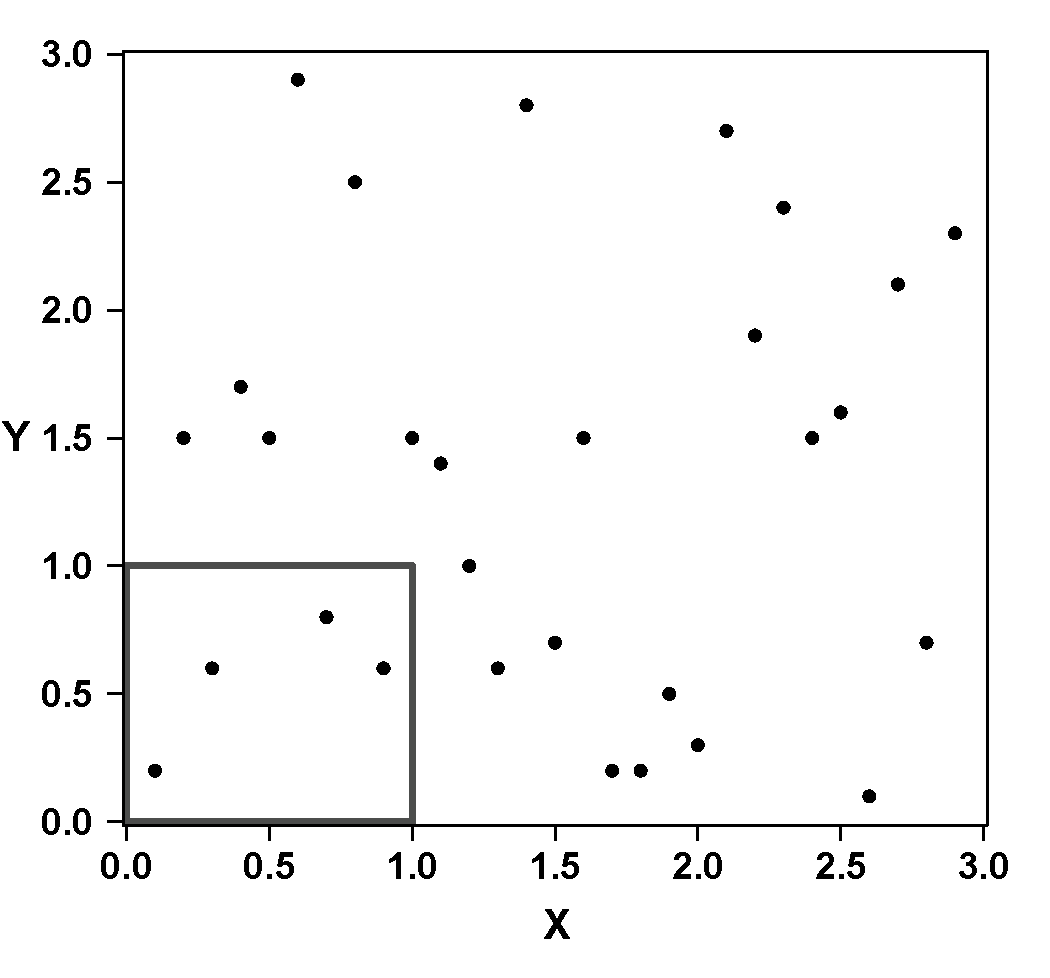
\includegraphics[width=0.28\textwidth]{./images/curse2Dsparse_BW.pdf}}&
\subfigure[]{\label{fig:curse3Dsparse}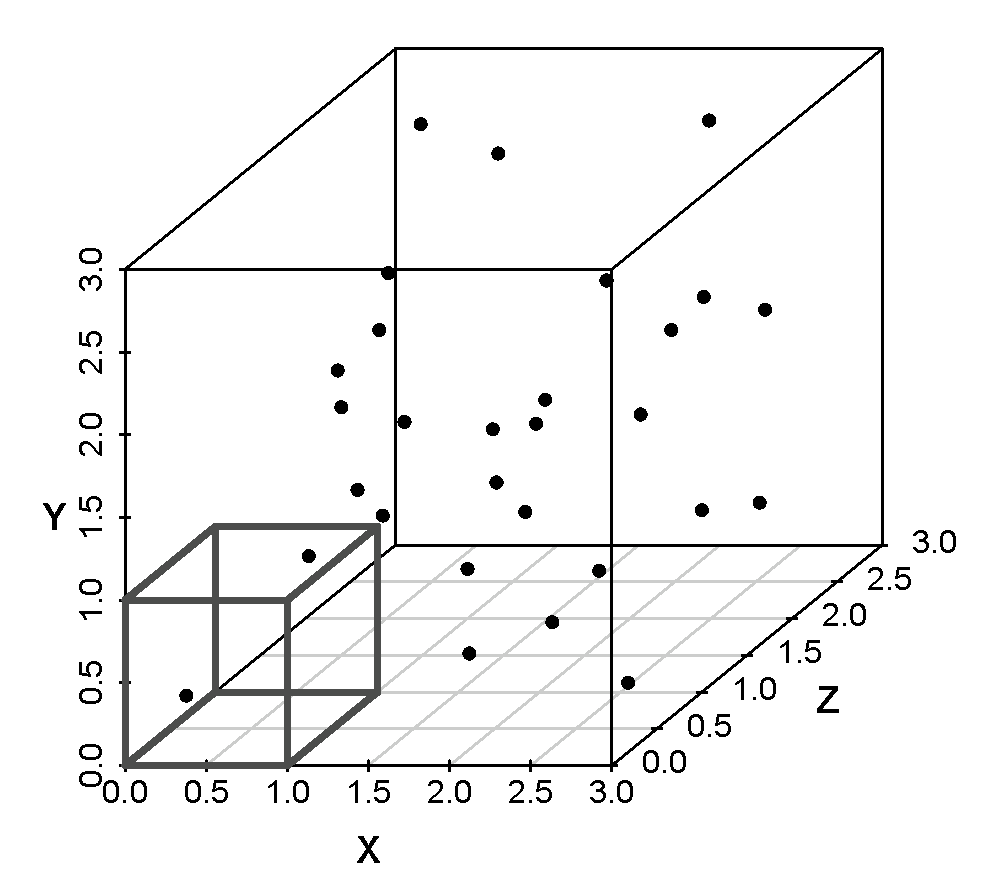
\includegraphics[width=0.28\textwidth]{./images/curse3Dsparse_BW.pdf}}\\
~  & 
\subfigure[]{\label{fig:curse2Ddense}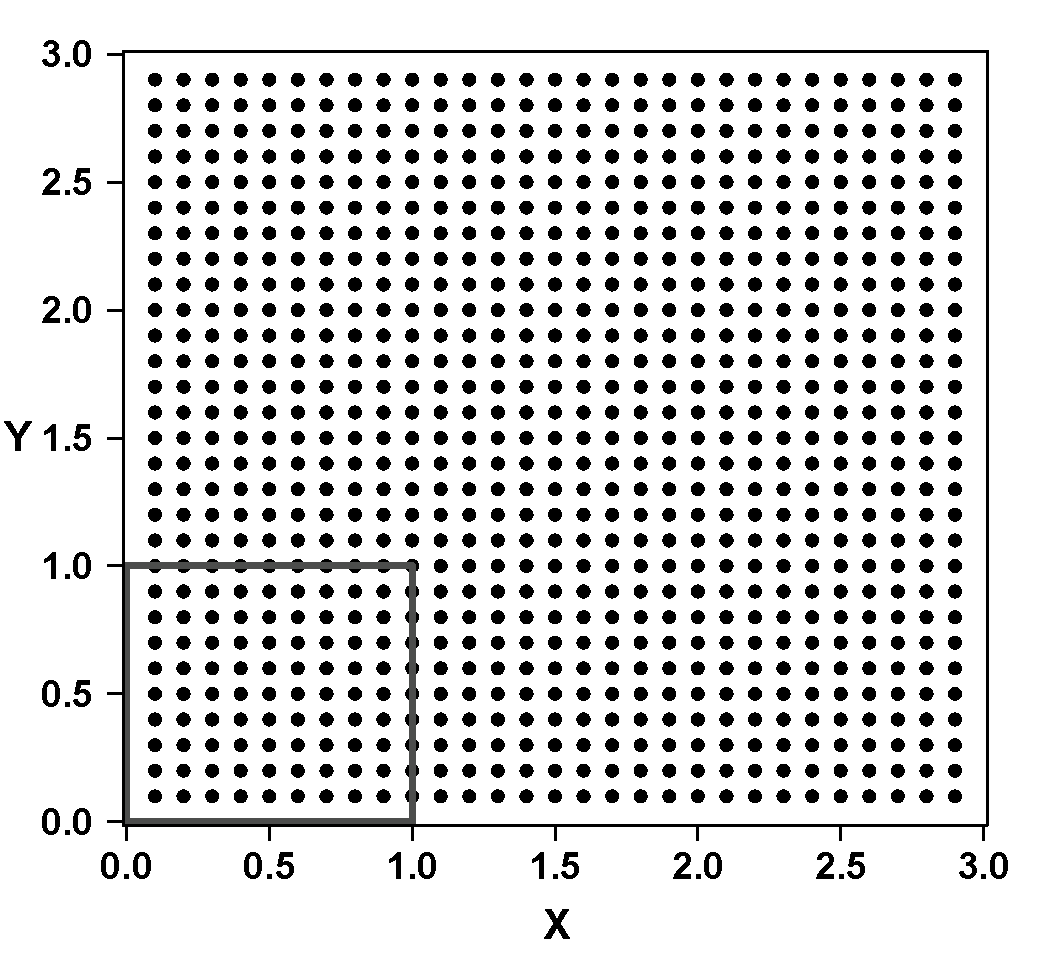
\includegraphics[width=0.28\textwidth]{./images/curse2Ddense_BW.pdf}}&
\subfigure[]{\label{fig:curse3Ddense}\includegraphics[width=0.28\textwidth]{./images/curse3Ddense_BW.pdf}}
\end{tabular}
\caption{Figures (d) and (e) illustrate the cost we must incur if we wish to maintain the density of the instances in the feature space as the dimensionality of the feature space increases.}
\label{fig:curseofdimen}
\end{figure}
\end{frame} 

\begin{frame} 
\begin{itemize}
\item During our discussion of feature selection approaches it will be useful to distinguish between different classes of descriptive features:
\begin{enumerate}
	\item \alert{Predictive}
	\item \alert{Interacting}
	\item \alert{Redundant}	
	\item \alert{Irrelevant}
\end{enumerate}
\end{itemize}
\end{frame} 

\begin{frame} 
\begin{itemize}
\item When framed as a local search problem feature selection is defined in terms of an iterative process consisting of the following stages:
\begin{enumerate}
\item \alert{Subset Generation}
\item \alert{Subset Selection}
\item \alert{Termination Condition}
\end{enumerate}
\item The search can move through the search space in a number of ways:
\begin{itemize}
\item \alert{Forward sequential selection}
\item \alert{Backward sequential selection}
\end{itemize}
\end{itemize}
\end{frame} 

\begin{frame} 
\begin{figure}
	\includegraphics[width=\textwidth]{./images/FeatureSubsetSpace.pdf}
	\caption{Feature Subset Space for a dataset with 3 features $X$, $Y$, $Z$.}
	\label{fig:featureSubsetSpace}
\end{figure}
\end{frame} 

\begin{frame} [plain]
\begin{figure}
	\includegraphics[width=\textwidth]{./images/FeatureSelectionProcess_BW.pdf}
	\caption{The process of model induction with feature selection.}
	\label{fig:mlprocessfeatureselection}
\end{figure}
\end{frame} 

\SectionSlideShortHeader{Efficient Memory Search}{Efficiency}

\begin{frame}
\begin{itemize}
\item Assuming that the training set will remain relatively stable it is possible to speed up the prediction speed of a nearest neighbor model by investing in some one-off computation to create an index of the instances that enables efficient retrieval of the nearest neighbors. 
\item The \alert{k-d tree}, which is short for k-dimensional tree, is one of the best known of these indexes.
\end{itemize}
\end{frame} 

\begin{frame} 
\begin{example}
Let's build a k-d tree for the college athlete dataset 

\begin{table}[htb]
\caption{The speed and agility ratings for 22 college athletes labelled with the decisions for whether they were drafted or not. }
\label{table:kddataset}
\centering
\begin{footnotesize}
\begin{tabular}{cc}
		\hline
			\begin{minipage}{0.45\textwidth}
				\centering
				\begin{footnotesize}
					\begin{tabular}[ht]{cccc} 
\textbf{ID}	 & \textbf{Speed} & \textbf{Agility} & \textbf{Draft}\\
\hline
1 & 2.50 & 6.00 & No\\
2 & 3.75 & 8.00 & No\\
3 & 2.25 & 5.50 & No\\
4 & 3.25 & 8.25 & No\\
5 & 2.75 & 7.50 & No\\
6 & 4.50 & 5.00 & No\\
7 & 3.50 & 5.25 & No\\
8 & 3.00 & 3.25 & No\\
9 & 4.00 & 4.00 & No\\
10 & 4.25 & 3.75 & No\\
11 & 2.00 & 2.00 & No\\
\hline
					\end{tabular}
				\end{footnotesize}
			\end{minipage}
			&
			\begin{minipage}{0.45\textwidth}
				\centering
					\begin{footnotesize}
					\begin{tabular}[ht]{cccc} 
\textbf{ID}	 & \textbf{Speed} & \textbf{Agility} & \textbf{Draft}\\
\hline
12 & 5.00 & 2.50 & No\\
13 & 8.25 & 8.50 & No\\
14 & 5.75 & 8.75 & Yes\\
15 & 4.75 & 6.25 & Yes\\
16 & 5.50 & 6.75 & Yes\\
17 & 5.25 & 9.50 & Yes\\
18 & 7.00 & 4.25 & Yes\\
19 & 7.50 & 8.00 & Yes\\
20 & 7.25 & 5.75 & Yes\\
21 & 6.75 & 3.00 & Yes\\
~& ~ & ~ & ~\\
\hline
				\end{tabular}
				\end{footnotesize}
			\end{minipage}\\
\end{tabular}
\end{footnotesize}
\end{table}
\end{example}
\end{frame} 

\begin{frame} [plain]
\begin{example}
\begin{center}
\textbf{First split on the \featN{Speed} feature}
\end{center}
\begin{figure}[htb]
	\begin{center}
\subfigure[]{\label{fig:kdtreeexam1a}\includegraphics[width=0.59\textwidth]{./images/kdtree_1st_level_simplified.pdf}}
\subfigure[]{\label{fig:kdtreeexam1b}\includegraphics[width=0.4\textwidth]{./images/kdtree_fs_1.pdf}} 
	\end{center}
       \caption{The k-d tree generated, for the dataset in Table \ourRef{table:kddataset} after the initial split using the \featN{Speed} feature. (b) the partitioning of the feature space by the k-d tree in (a).}	
	\label{fig:kdtreeexam1}
\end{figure}
\end{example}
\end{frame} 

 \begin{frame} [plain]
 \begin{example}
 \begin{center}
\textbf{Next split on the \featN{Agility} feature}
\end{center}
\begin{figure}[htb]
	\begin{center}
\subfigure[]{\label{fig:kdtreeexam2a}\includegraphics[width=0.59\textwidth]{./images/kdtree_2nd_level_simplified.pdf}} 
\subfigure[]{\label{fig:kdtreeexam2b}\includegraphics[width=0.4\textwidth]{./images/kdtree_fs_2.pdf}}		
	\end{center}
       \caption{(a) the k-d tree after the dataset at the left child of the root has been split using the \featN{Agility} feature with a threshold of $5.5$. (b) the partitioning of the feature space by the k-d tree in (a)}	
	\label{fig:kdtreeexam2}
\end{figure}
\end{example}
\end{frame} 

\begin{frame} [plain]
\begin{example}
\begin{center}
\textbf{After completing the tree building process}
\end{center}
\begin{figure}[htb]
	\begin{center}
\subfigure[]{\label{fig:kdtreeexam2a}\includegraphics[width=0.59\textwidth]{./images/kdtree_complete_narrow.pdf}} 
\subfigure[]{\label{fig:kdtreeexam2b}\includegraphics[width=0.4\textwidth]{./images/kdtree_fs_3.pdf}}		
	\end{center}
       \caption{(a) The complete k-d tree generated, for the dataset in Table \ourRef{table:kddataset}. (b) the partitioning of the feature space by the k-d tree in (a)}	
	\label{fig:kdtreeexam3}
\end{figure}
\end{example}
\end{frame} 

\begin{frame} 
\begin{example}
\begin{center}
\textbf{Finding neighbors for query \featN{Speed}$=6$, \featN{Agility}$=3.5$.}
\end{center}
\begin{figure}[htb]
	\begin{center}
\begin{tabular}{cc}
\subfigure[]{\label{fig:kdtreeexam4a}\includegraphics[width=0.6\textwidth]{./images/kdtree_complete_retrieval1_narrow_simplified.pdf}}&
\subfigure[]{\label{fig:kdtreeexam4b}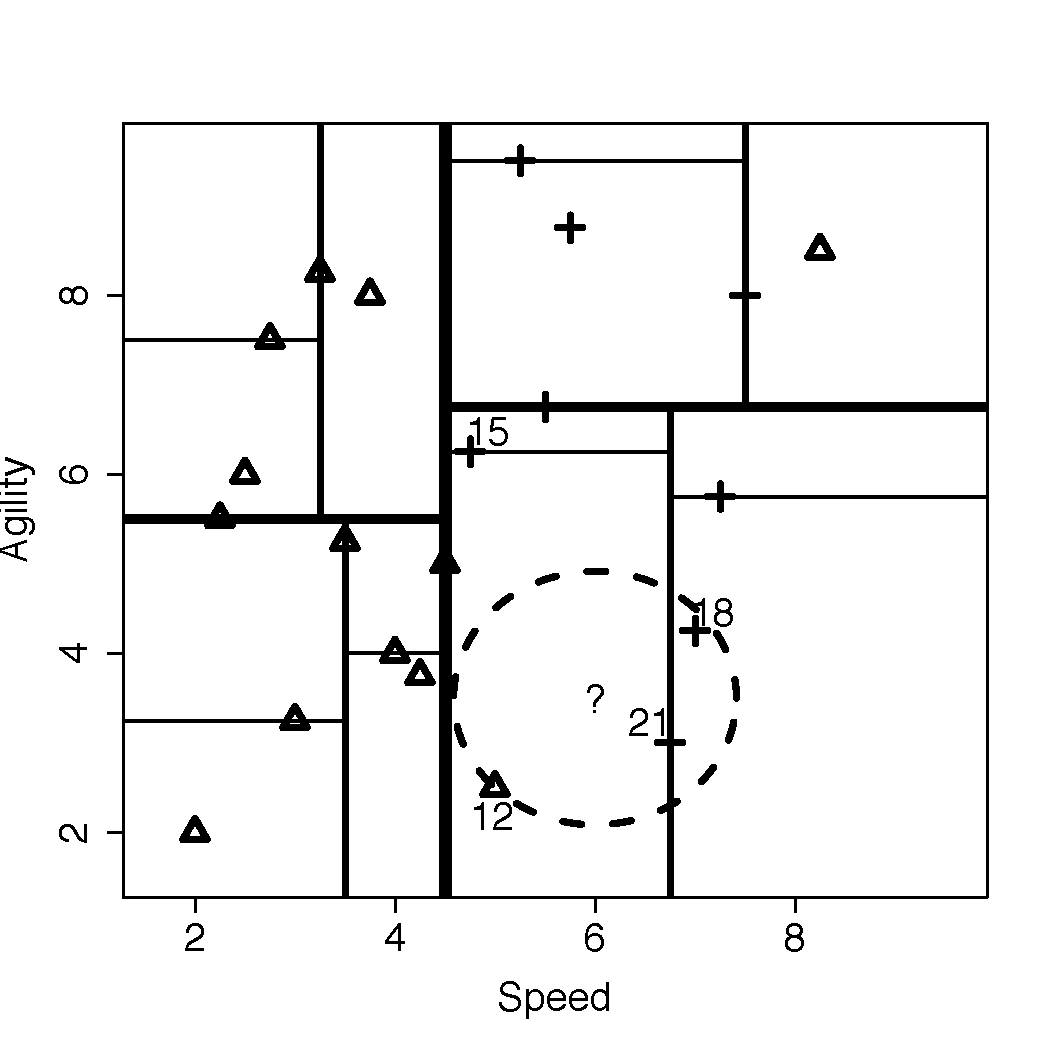
\includegraphics[width=0.3\textwidth]{./images/kdtree_fs_4_labelled.pdf}}		
	\end{tabular}
	\end{center}
       \caption{(a) the path taken from the root node to a leaf node when we search the tree. (b) the location of the query in the feature space is represented by the ? and the target hypersphere defining the region that must contain the true nearest neighbor.}	
	\label{fig:kdtreeexam4}
\end{figure}
\end{example}
\end{frame} 

\begin{frame} 
\begin{example}
\begin{center}
\textbf{Finding neighbors for query \featN{Speed}$=6$, \featN{Agility}$=3.5$.}
\end{center}
\begin{figure}[htb]
	\begin{center}
\begin{tabular}{cc}
\subfigure[]{\label{fig:kdtreeexam5a}\includegraphics[width=0.6\textwidth]{./images/kdtree_retrieval2_labelled_BW.pdf}}&
\subfigure[]{\label{fig:kdtreeexam5b}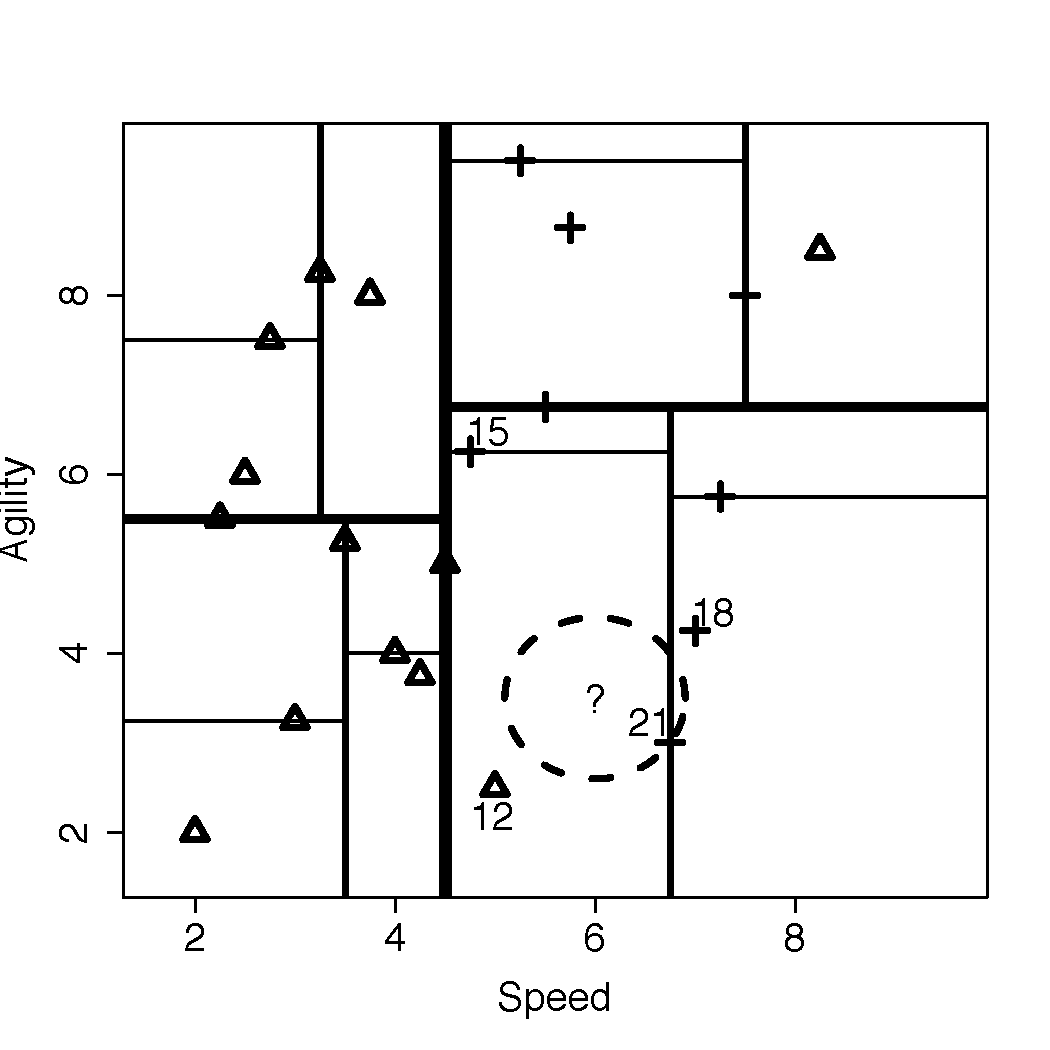
\includegraphics[width=0.3\textwidth]{./images/kdtree_fs_5_labelled.pdf}}		
	\end{tabular}
	\end{center}
       \caption{(a) the state of the retrieval process after instance $\mathbf{d}_{21}$ has been stored as \emph{current-best}. (b) the dashed circle illustrates the extent of the target hypersphere after \emph{current-best-distance} has been updated.}	
	\label{fig:kdtreeexam5}
\end{figure}
\end{example}
\end{frame} 

\begin{frame} 
\begin{example} 
\begin{figure}[htb]
	\begin{center}
\includegraphics[width=0.9\textwidth]{./images/kdtree_complete_retrieval3_simplified.pdf}
	\end{center}
       \caption{The greyed out branches indicate the portions of the k-d tree pruned from the search. The node with the bold outline represents the instance ($\mathbf{d}_{21}$) that was returned as the nearest neighbor to the query.}	
	\label{fig:kdtreeexam6}
\end{figure}
\end{example} 
\end{frame} 

\SectionSlide{Summary}


\begin{frame}
\begin{itemize}
\item Nearest neighbor models are very sensitive to noise in the target feature the easiest way to solve this problem is to employ a \keyword{\textit{k} nearest neighbor}.
\item \keyword{Normalization} techniques should almost always be applied when nearest neighbor models are used. 
\item It is easy to adapt a nearest neighbor model to \keyword{continuous targets}. 
\item There are many different measures of \keyword{similarity}. 
\item \keyword{Feature selection} is a particularly important process for nearest neighbor algorithms it alleviates the \keyword{curse of dimensionality}.  
\item As the number of instances becomes large, a nearest neighbor model will become slower---techniques such as the \keyword{\textit{k-d} tree} can help with this issue. 
\end{itemize}
\end{frame}

\begin{frame}
	\tableofcontents
\end{frame}

\end{document}
